%!TEX root = ms.tex
\section{Performance of the selectors}
\label{sec:simulation}
\subsection{Some other selectors}
In this section we use computer simulations to explore the behavior of different criteria when used for model selection under linear restrictions (variable selection and general linear restrictions). In addition to the criteria already discussed, we also consider two other well-known criteria: 
\begin{equation*}
\text{BIC}(k) = n \log\left( \frac{\text{RSS}(k)}{n} \right) +\log(n) k
%\label{eq:bic}
\end{equation*}
\citep{schwarz1978estimating}, and generalized cross-validation (GCV)
\begin{equation}
\text{GCV}(k) = \text{RSS}(k)\frac{n^2}{(n-k)^2}.
\label{eq:gcv_subsetselection}
\end{equation}
BIC is a consistent criterion, in the sense that under some conditions, if the true model is among the candidate models, the probability of selecting the true model approaches one, as the sample size becomes infinite. GCV, derived by \citet{craven1978smoothing} in the context of smoothing, is equivalent to the mean square over degrees of freedom criterion proposed by \citet{tukey1967discussion}. By comparing the expressions of \eqref{eq:gcv_subsetselection} and \eqref{eq:sp_subsetselection}, GCV and S$_p$ only differ by a multiplicative factor of $1 + k / [(n-k)(n-1)]$.

By analogy to the criteria discussed in Section \ref{sec:ic_fixedx} and \ref{sec:ic_randomx}, if we substitute $k=p-m$ into the expressions of BIC$(k)$ and GCV$(k)$, we obtain their corresponding expressions for general linear restrictions BIC$(R,r)$ and GCV$(R,r)$, respectively. We also consider two types of the cross-validation (CV): 10-fold CV (denoted as 10FCV) and leave-one-out CV (LOOCV). The LOOCV is based on the PRESS(k) statistic for the variable selection problem and PRESS(R,r) for the general restriction problem.


\subsection{Random-X}
We first consider the variable selection problem. The candidate models include the predictors of $X$ in a nested fashion, i.e. the candidate model of size $k$ includes the first $k$ columns of $X$ ($X_1,\cdots,X_k$). We describe the simulation settings reported here; description of and results from all other settings (243 configurations in total) can be found in the Online Supplemental Material\footnote{\url{https://github.com/sentian/RAICc}}, where we also provide the code to reproduce all of the simulation results in this paper. The sample sizes considered are $n\in\{40, 1000\}$, with number of predictors $p=n-1$, being close to the sample size. Predictors exhibit moderate correlation with each other of an AR(1) type (see the Online Supplemental material for further details), and the strength of the overall regression is characterized as either low (average $R^2$ on the set of true predictors roughly $20\%$) or high (average $R^2$ on the set of true predictors roughly $90\%$). The true model is either sparse (with six nonzero slopes) or dense (with $p$ nonzero slopes exhibiting diminishing strengths of coefficients; \citealp{Taddy2017}). The design matrix $X$ is random. In each replication, we generate a matrix $X$ such that the rows $x_i$ ($i=1,\cdots,n$) are drawn from a $p$-dimensional multivariate normal distribution with mean zero and covariance matrix $\Sigma_0$, and we draw the response $y$ from the conditional distribution of $y|X$ based on \eqref{eq:truemodel}. The entire process is repeated $1000$ times. 

We consider the following metrics to evaluate the fit. The values of each criterion over all of the simulation runs are plotted using side-by-side boxplots, with the average value over the simulation runs given below the boxplot for the corresponding criterion.
\begin{itemize}
  \item Root mean squared error for random-X:
  \begin{equation*}
    \text{RMSER} = \sqrt{ E_{X^n} \lVert X^n\hat\beta-X^n\beta_0 \rVert_2^2 } =  \sqrt{ (\hat{\beta}-\beta_0)^T \Sigma_0 (\hat{\beta}-\beta_0) }.
  \end{equation*} 

  \item KL discrepancy for random-X \eqref{eq:KLR} in the log scale (denoted as logKLR).

  \item Size of the subset selected for variable selection problem, and number of restrictions in the selected model for general restriction problem.
\end{itemize}

The results are presented in Figures \ref{fig:subsetselection_randomx_hsnr_largep} and \ref{fig:subsetselection_randomx_lsnr_largep}. We find that RAICc provides the best predictive performance and the sparsest subset while rarely underfitting, compared to other information criteria designed for random-X, including RC$_p$ and S$_p$. The underperformance of RC$_p$ and S$_p$ is due to overfitting. S$_p$, as an estimate of the squared prediction error, is a product of an unlogged residual sum of squares and a penalty term that is increasing in $k$. This results in higher variability in S$_p$ for models that overfit, thereby potentially increasing the chances for spurious minima of these criteria at models that drastically overfit. In RAICc, on the other hand, the residual sum of squares is logged, thereby stabilizing the variance and avoiding the problem. RC$_p$ drastically overfits in all scenarios, reflecting the price of estimating $\sigma_0^2$ using the full model, especially when $p$ is close to $n$. S$_p$, on the other hand, estimates $\sigma_0^2$ using the candidate model, which mitigates the problem. Nevertheless, S$_p$ also can sometimes strongly overfit, but only when $n$ is small. Even for large $n$, S$_p$ selects slightly larger subsets on average than does RAICc. 

We also note that information criteria designed for random-X generally perform better than their counterparts for the fixed-X case. Both C$_p$ and FPE are largely outperformed by RC$_p$ and S$_p$, respectively. The advantage of RAICc over AICc is statistically significant in most scenarios, based on the Wilcoxon signed-rank test (the $p$-value for the test comparing the criteria for RAICc and AICc is given above the first two boxes in the first two columns of the table), but is not obvious in a practical sense. The only place that we see an advantage of AICc is for \{Dense model, $n=40$ and high signal\}. In this scenario, a model with many predictors with nonzero slopes can predict well, but that advantage disappears when there is a relatively weak signal, as in that situation the added noise from including predictors with small slopes cannot be overcome by a small error variance. 

We further note that choosing the appropriate family of information criteria (the KL-based AICc and RAICc) is more important than choosing the information criteria designed for the underlying designs of $X$. AICc, despite being designed for fixed-X, outperforms RC$_p$ and S$_p$, which are designed for random-X in all of the scenarios, in terms of both predictive performance and providing sparse results. The KL-based criteria have a clear advantage compared to the squared-error based criteria.

Finally, we note some other findings that have been discussed previously in the literature. Despite its apparently strong penalty, BIC often chooses the model using all predictors when $n$ is close to $p$, as discussed in \citet{hurvich1989regression} and \citet{baraud2009gaussian}. We also see that even though GCV has a similar penalty term as S$_p$, it is more likely to suffer from overfitting. Unlike S$_p$, GCV can sometimes drastically overfit even when $n$ is large. The overfitting problem of GCV was also observed in the context of smoothing by \citet{hurvich1998smoothing}. We further find that 10-fold CV performs better than LOOCV, the latter of which sometimes drastically overfits. The tendency of LOOCV to strongly overfit was noted by \citet{scott1987biased} and \citet{hall1991local} in the context of smoothing. \citet{zhang2015cross} showed that when applied as selection rules, the larger validation set used by 10-fold CV can better distinguish the candidate models than can LOOCV, and this results in a model with smaller predictive error. RAICc performs better than 10-fold CV for small $n$, and performs similarly for large $n$. Computationally, 10-fold CV is ten times more expensive compared to RAICc, and since the split of validation samples is random, 10-fold CV can select different subsets if applied multiple times on the same dataset; that is, the result of 10-fold CV is not reproducible. The fact that LOOCV provides better estimate of the test error while being outperformed by 10-fold CV, further emphasizes the difference between the goal of providing the best estimate of the test error, and the goal of selecting the models with the best predictive performance. Clearly, KL-based criteria (AICc and RAICc) bridge the gap between the two goals more effectively than the squared-error based criteria (including cross-validation).

In a related study by \citet{leeb2008evaluation}, the author found that S$_p$ and GCV outperform AICc under random-X, but those results are not directly comparable to ours. That paper did not consider the case where $p$ is extremely close to $n$, which is the scenario that most separates the performances of the different criteria. 

\begin{figure}[!ht]
  \centering
  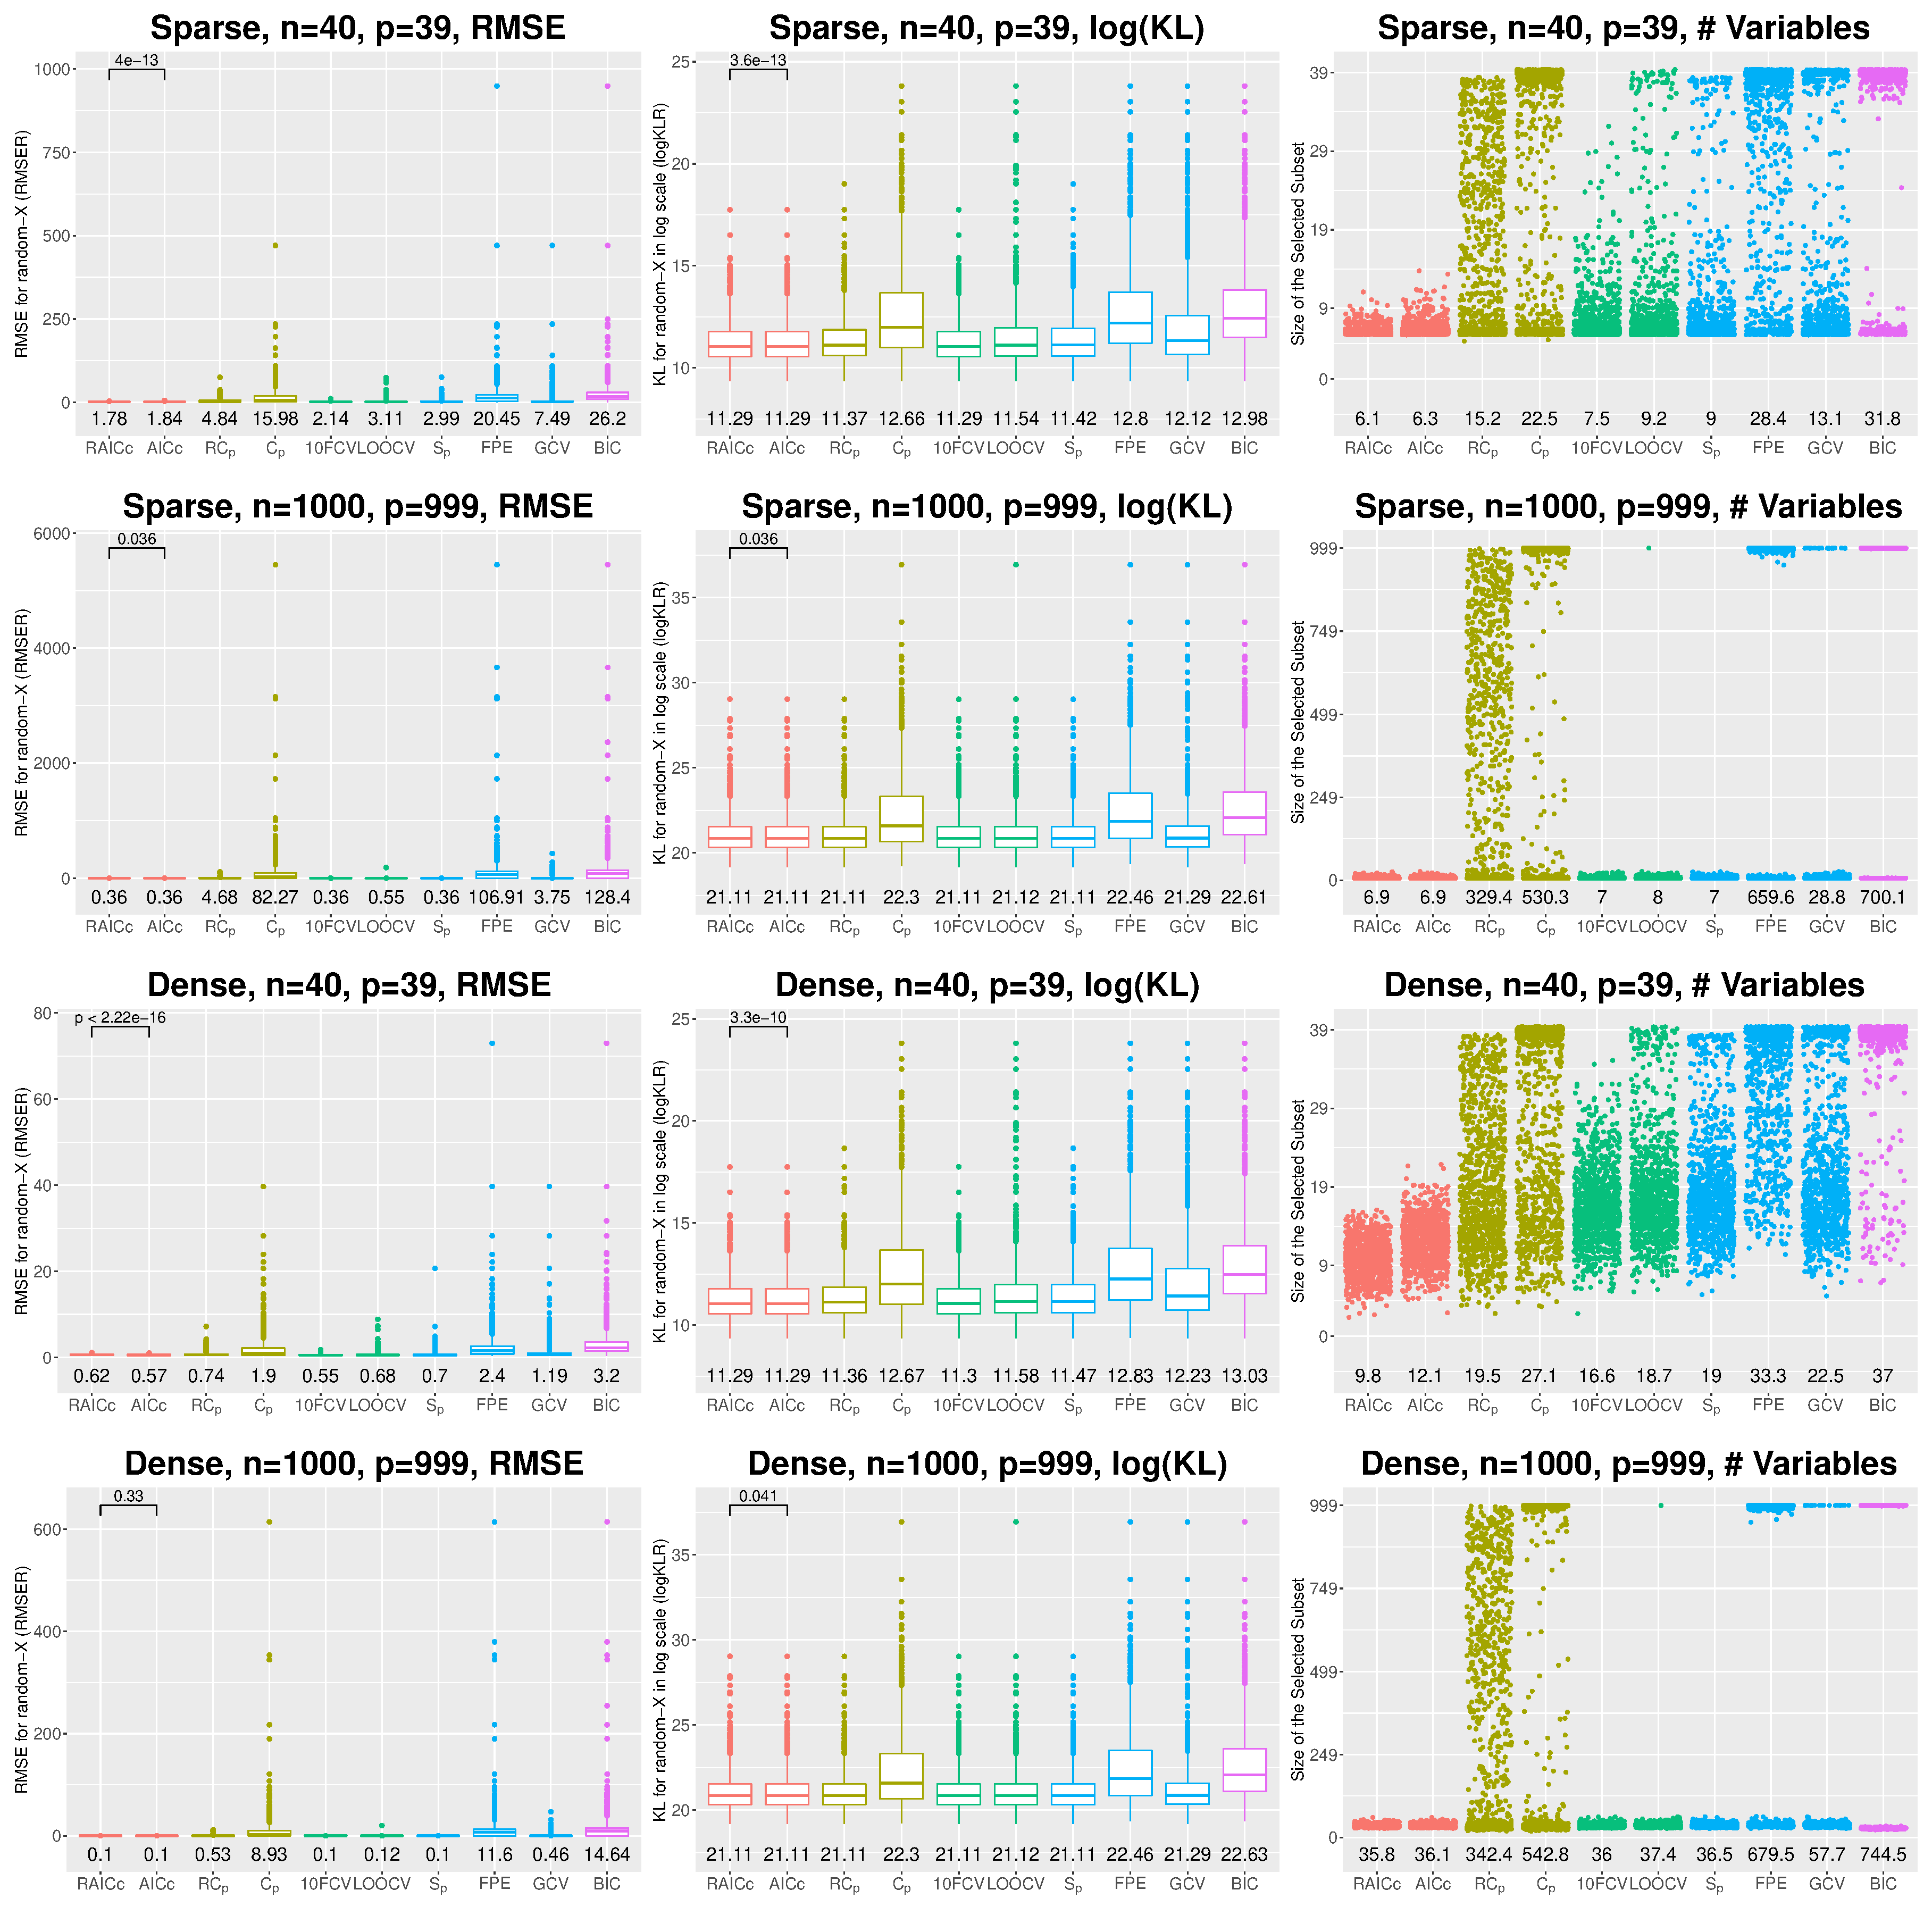
\includegraphics[width=\textwidth]{figures/main/randomx_VS_hsnr.eps}
  \caption{Results of simulations for variable selection. Random-X, high signal and $\rho=0.5$. The Sparse and Dense models correspond to the VS-Ex2 and VS-Ex3 configurations (details are given in the Online Supplemental Material). The first column refers to RMSE, the second column corresponds to KL discrepancy (in log scale), and the third column gives the number of variables in the selected model with nonzero slopes, jittered horizontally and vertically, so the number of models with that number of nonzero slopes can be ascertained more easily. The mean values of the evaluation metrics for each criterion are presented at the bottom of each graph. The p-values of the Wilcoxon signed-rank test (paired and two-sided) for comparing RAICc and AICc are also presented.}
  \label{fig:subsetselection_randomx_hsnr_largep}
\end{figure}


\begin{figure}[!ht]
  \centering
  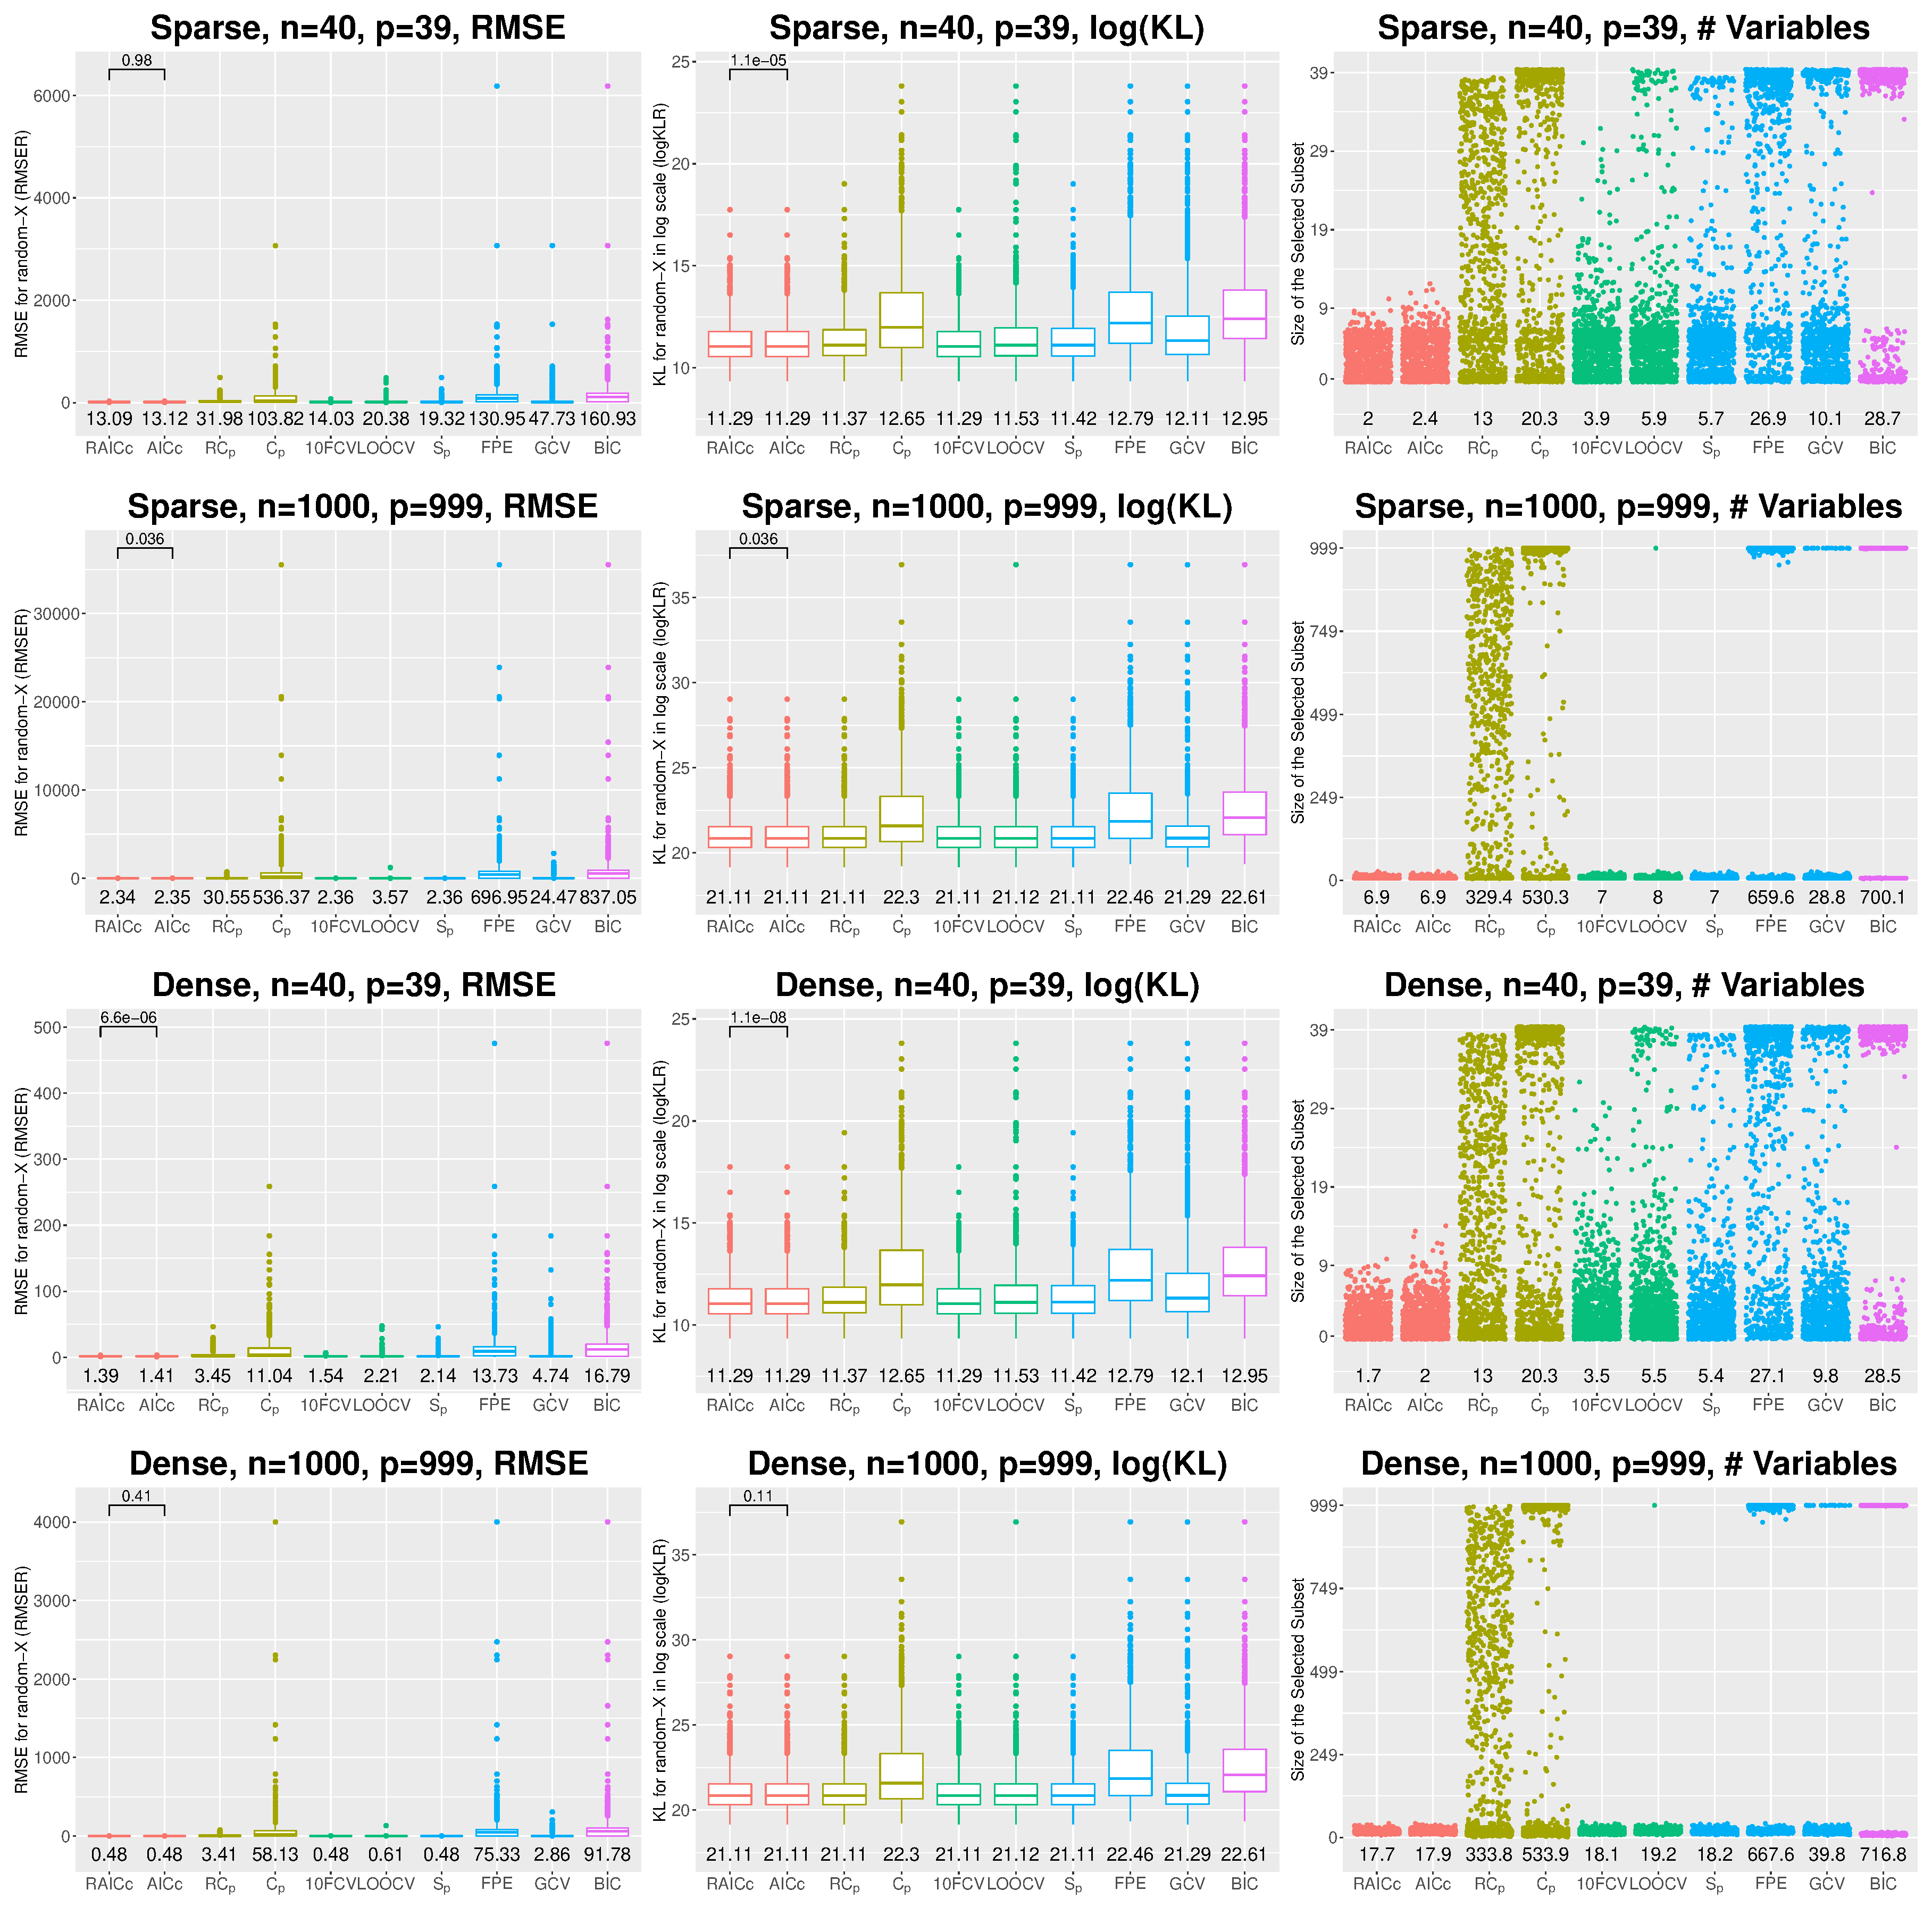
\includegraphics[width=\textwidth]{figures/main/randomx_VS_lsnr.eps}
  \caption{Results of simulations for variable selection. Random-X, low signal and $\rho=0.5$. }
  \label{fig:subsetselection_randomx_lsnr_largep}
\end{figure}

We next consider the general restriction problem. We take $\beta_0 = [2,2,2,1,1,1]^T$, $n\in\{10,40\}$, moderate correlations between the predictors, and either high or low signal levels. The candidate models are constructed in the following way. We consider a set of restrictions: $\beta_1=\beta_4$, $\beta_1=2\beta_2$, $\beta_1=\beta_2$, $\beta_2=\beta_3$, $\beta_4=\beta_5$, $\beta_5=\beta_6$, where the last four restrictions hold for our choice of $\beta_0$. We then consider all of the possible subsets of the six restrictions, resulting in $64$ candidate models in total. The detailed configurations and complete results for this and other examples of the general restriction problem ($54$ scenarios in total) are given in the Online Supplemental Material. 

We see from Figure \ref{fig:generalrestriction_randomx} that differences in performance between the criteria are less dramatic. This is not surprising, since for these models the number of parameters never approaches the sample size. Still, RAICc is consistently the best selection rule for small sample size $n$, and it is second-best for large $n$, where it is outperformed by BIC (note that BIC has a strong tendency to select too few restrictions when the sample is small, which corresponds to overfitting in the variable selection context). We also note an advantage of RAICc over AICc, with AICc having a stronger tendency to select too few restrictions.

\begin{figure}[!ht]
  \centering
  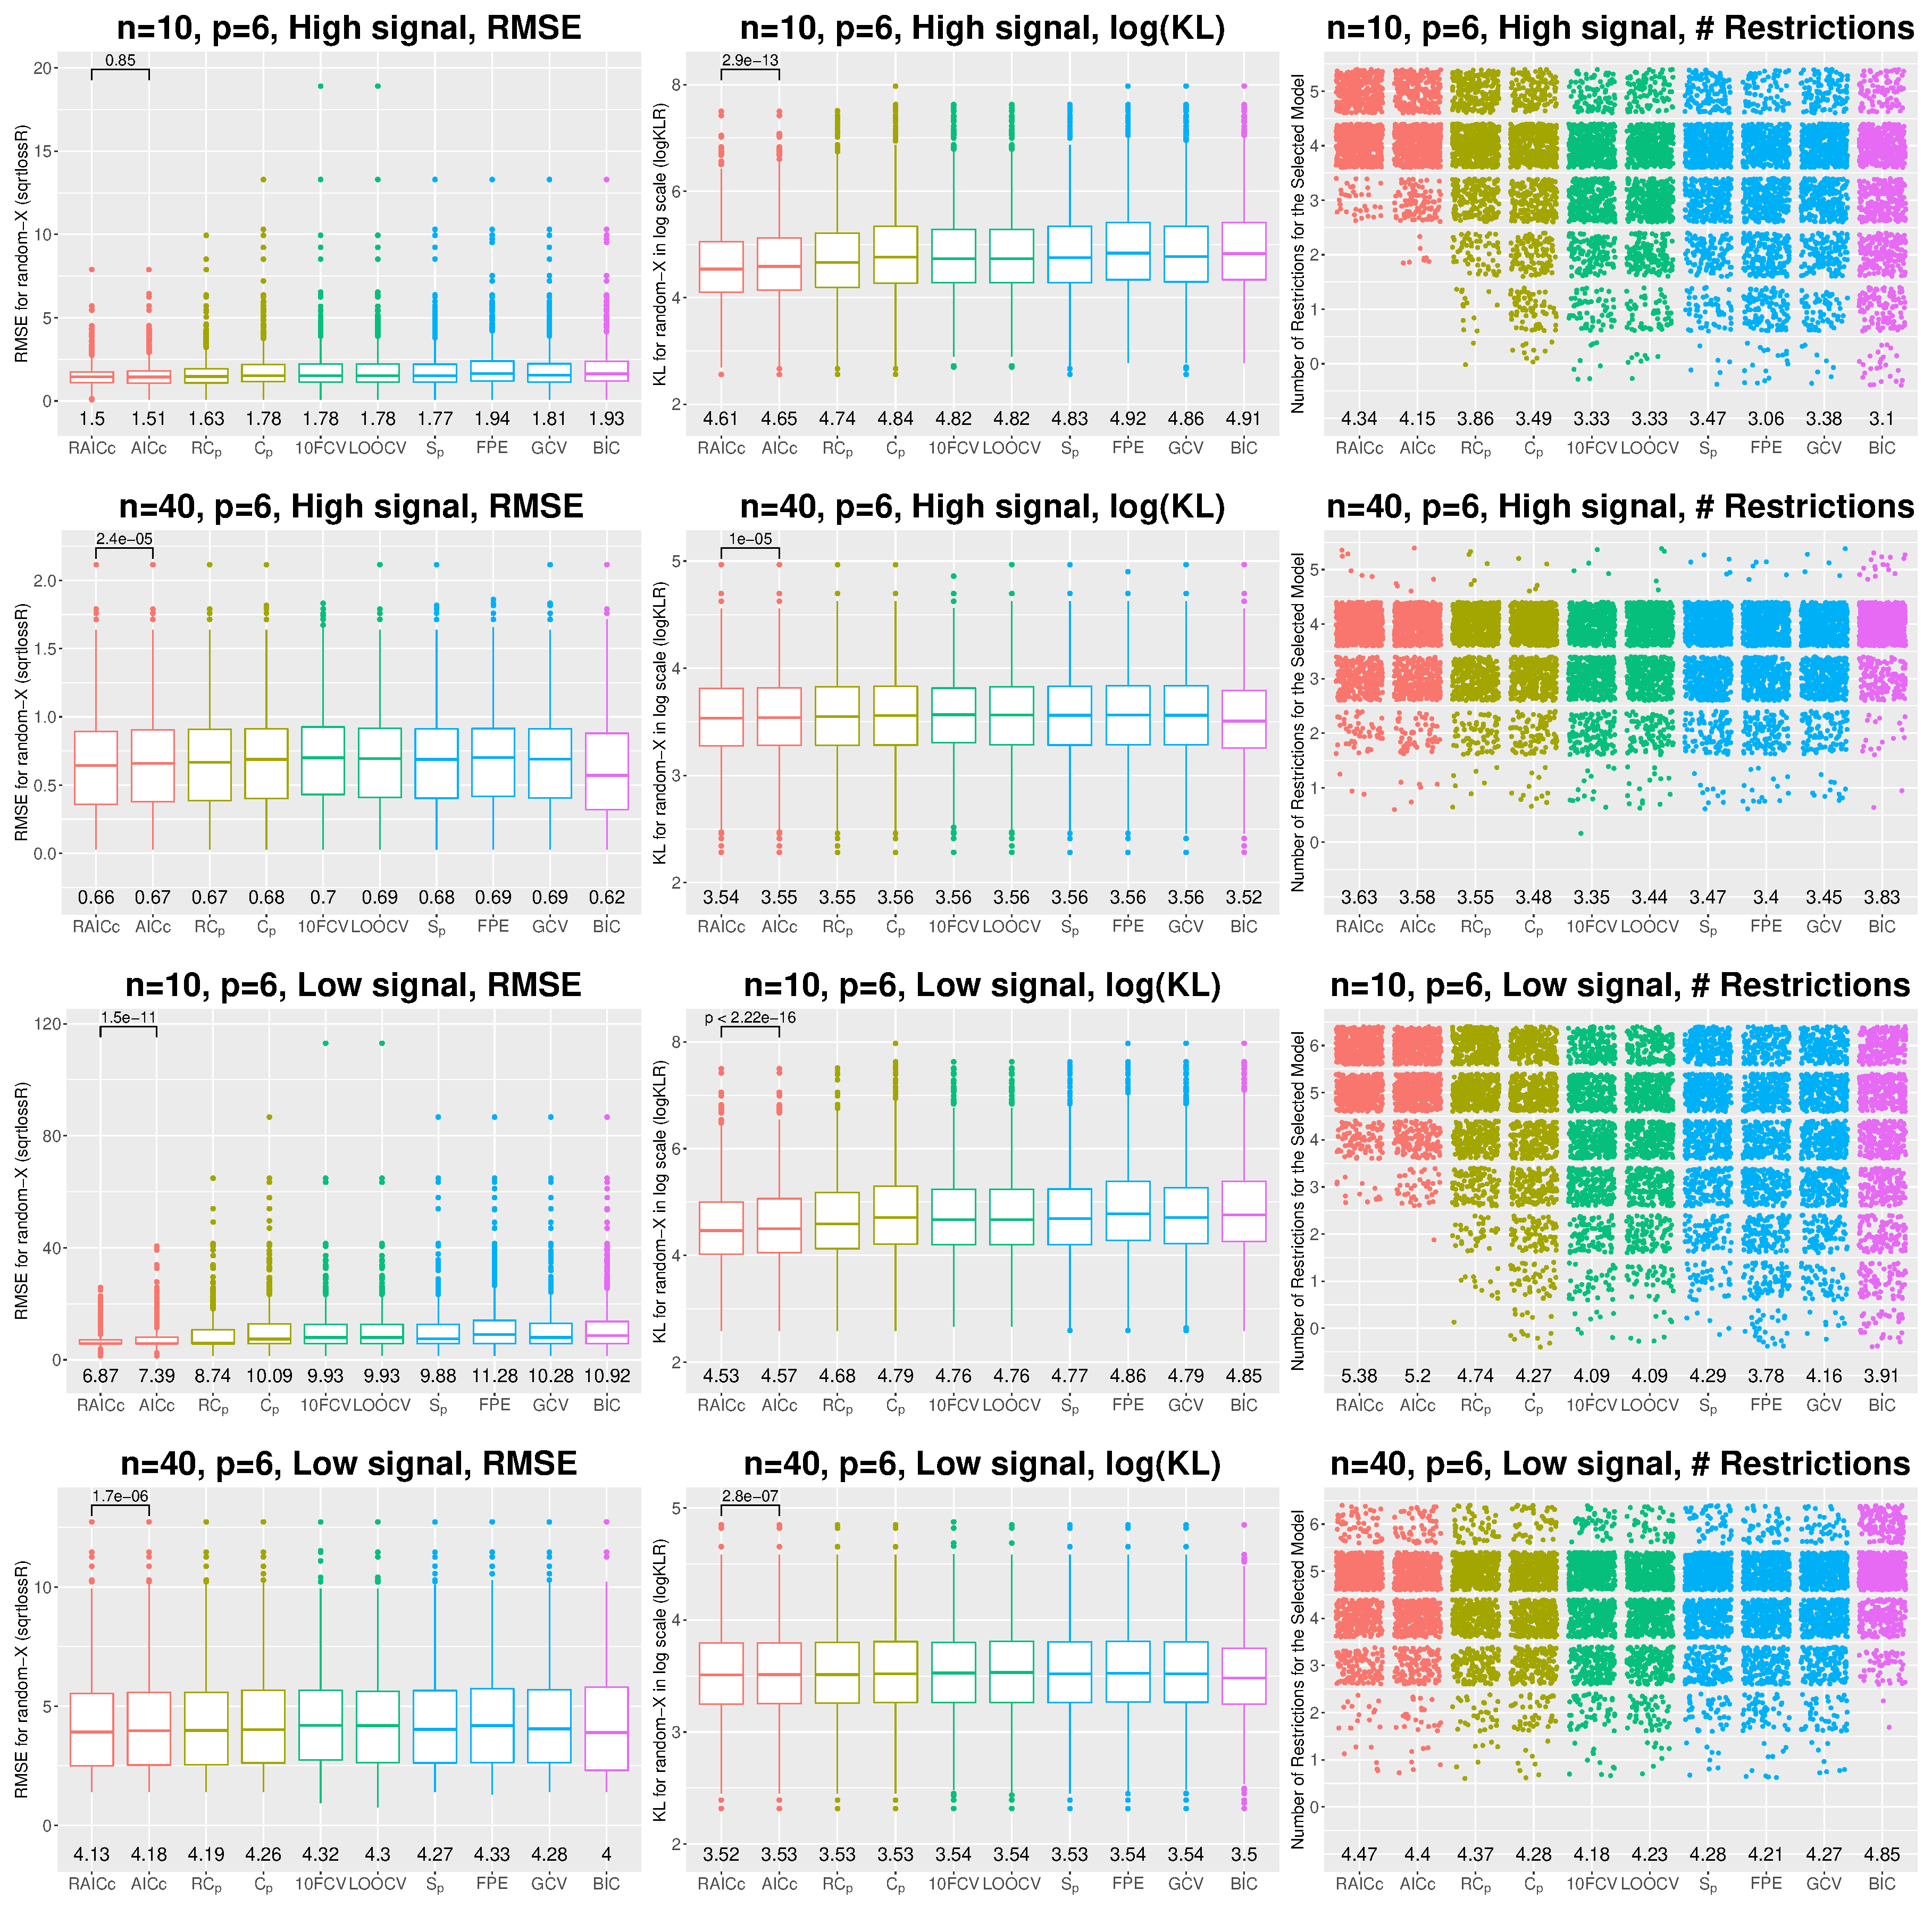
\includegraphics[width=\textwidth]{figures/main/randomx_GR-Ex1.eps}
  \caption{Results of simulations for general restrictions. Random-X, $\rho=0.5$. The configuration of the model is GR-Ex1 (details can be found in the Online Supplemental Material). Third column gives the number of restrictions in the selected models, jittered horizontally and vertically. }
  \label{fig:generalrestriction_randomx}
\end{figure}

Finally, we extend the general restriction example by including restrictions that force additional predictors to have zero coefficients (as in the variable selection problem). Besides the six restrictions specified, we also consider $\beta_i=0$ for $i=7,\cdots,p$ resulting in $p$ possible restrictions in total. The candidate models are formulated by excluding the restrictions in a nested fashion. We start from the model including all $p$ restrictions (corresponding to the null model), and the next model includes the $p-1$ restrictions except the first one $\beta_1=\beta_4$. The process is repeated until all restrictions are excluded (the full model including all predictors with arbitrary slopes) resulting in $p+1$ candidate models in total. The true coefficient vector is the same as that used in Figure \ref{fig:generalrestriction_randomx}, implying that the correct number of restrictions is $p-2$. We present the detailed configurations and complete results for this and other examples ($243$ scenarios in total) in the Online Supplemental Material. 

We see from Figure \ref{fig:subsetgeneral_randomx} that our findings for the variable selection problem also hold in this case. This is not surprising, since variable selection is just a special example of general restrictions, and in this scenario the set of candidate models includes ones where the number of parameters is close to the sample size. Thus, overall, RAICc and AICc are the best performers among all of the selectors. RAICc tends to provide the sparsest subset (or select more restrictions), while rarely underfitting, having a slight advantage over AICc in terms of predictive performance. 

\begin{figure}[!ht]
  \centering
  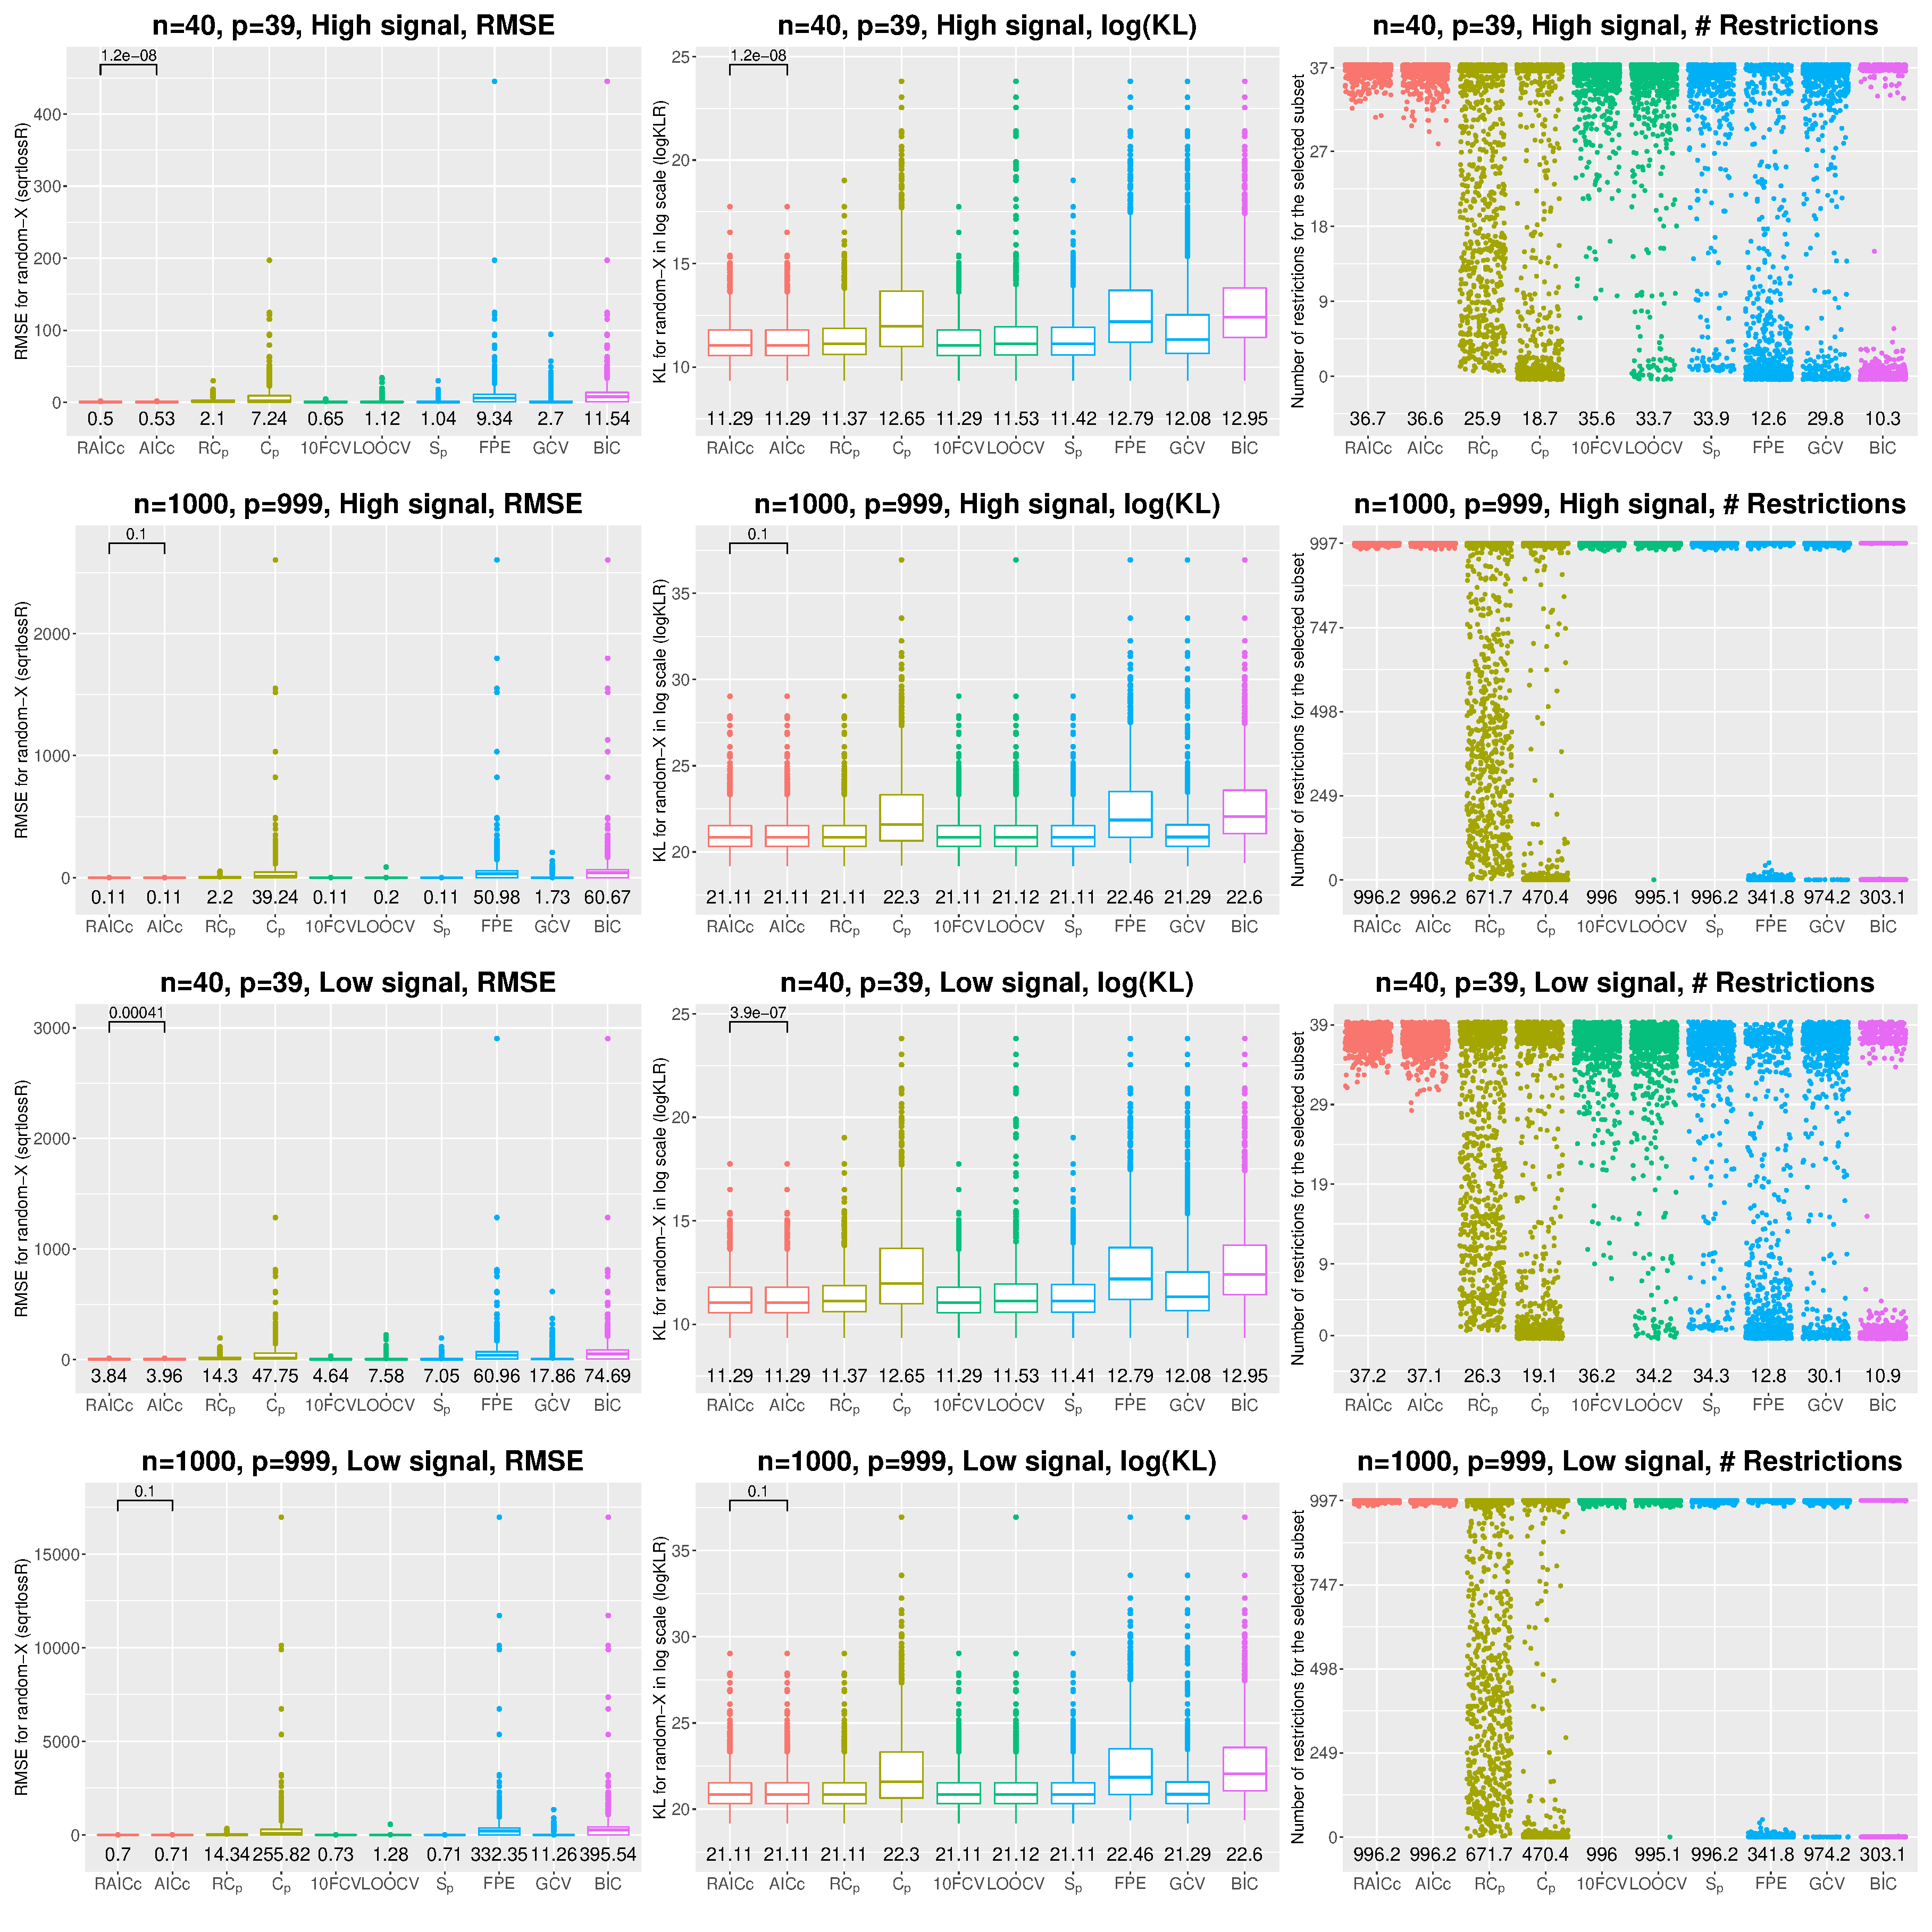
\includegraphics[width=\textwidth]{figures/main/randomx_GR-Ex4.eps}
  \caption{Results of simulations for general restrictions. Random-X, $\rho=0.5$. The configuration of the model is GR-Ex4 (details can be found in the Online Supplemental Material).}
  \label{fig:subsetgeneral_randomx}
\end{figure}

\iffalse
\subsubsection{Without a true model}
\begin{itemize}
	\item Omit: The configuration is the same as Sparse-Ex1, but with the 6-th predictor treated as missing for all the fitting procedures.
	\item Exponential: We take $\Sigma = I$. The responses are generated by $y_i=exp(4i/n) + \epsilon_i$, for $i=1,\cdots,n$, where $\epsilon_i$ are independent $\mathcal{N}(0, \sigma_0^2)$. 
\end{itemize}
	We consider a fixed trigonometric configuration of $X$ that is studied by \citet{Hurvich1991}, where $X$ is an $n$ by $p$ matrix with components defined by 
$$ x_{t, 2j-1} = \sin\left(\frac{2\pi j}{n}t\right),$$
and 
$$ x_{t,2j} = \cos\left(\frac{2\pi j}{n}t\right),$$
for $j=1,\cdots,p/2$ and $t=0,\cdots,n-1$. The responses are generated by $y_i=exp(4i/n) + \epsilon_i$, for $i=1,\cdots,n$, where $\epsilon_i$ are independent $\mathcal{N}(0, \sigma_0^2)$. 
\fi



\iffalse
\begin{figure}[!ht]
  \centering
  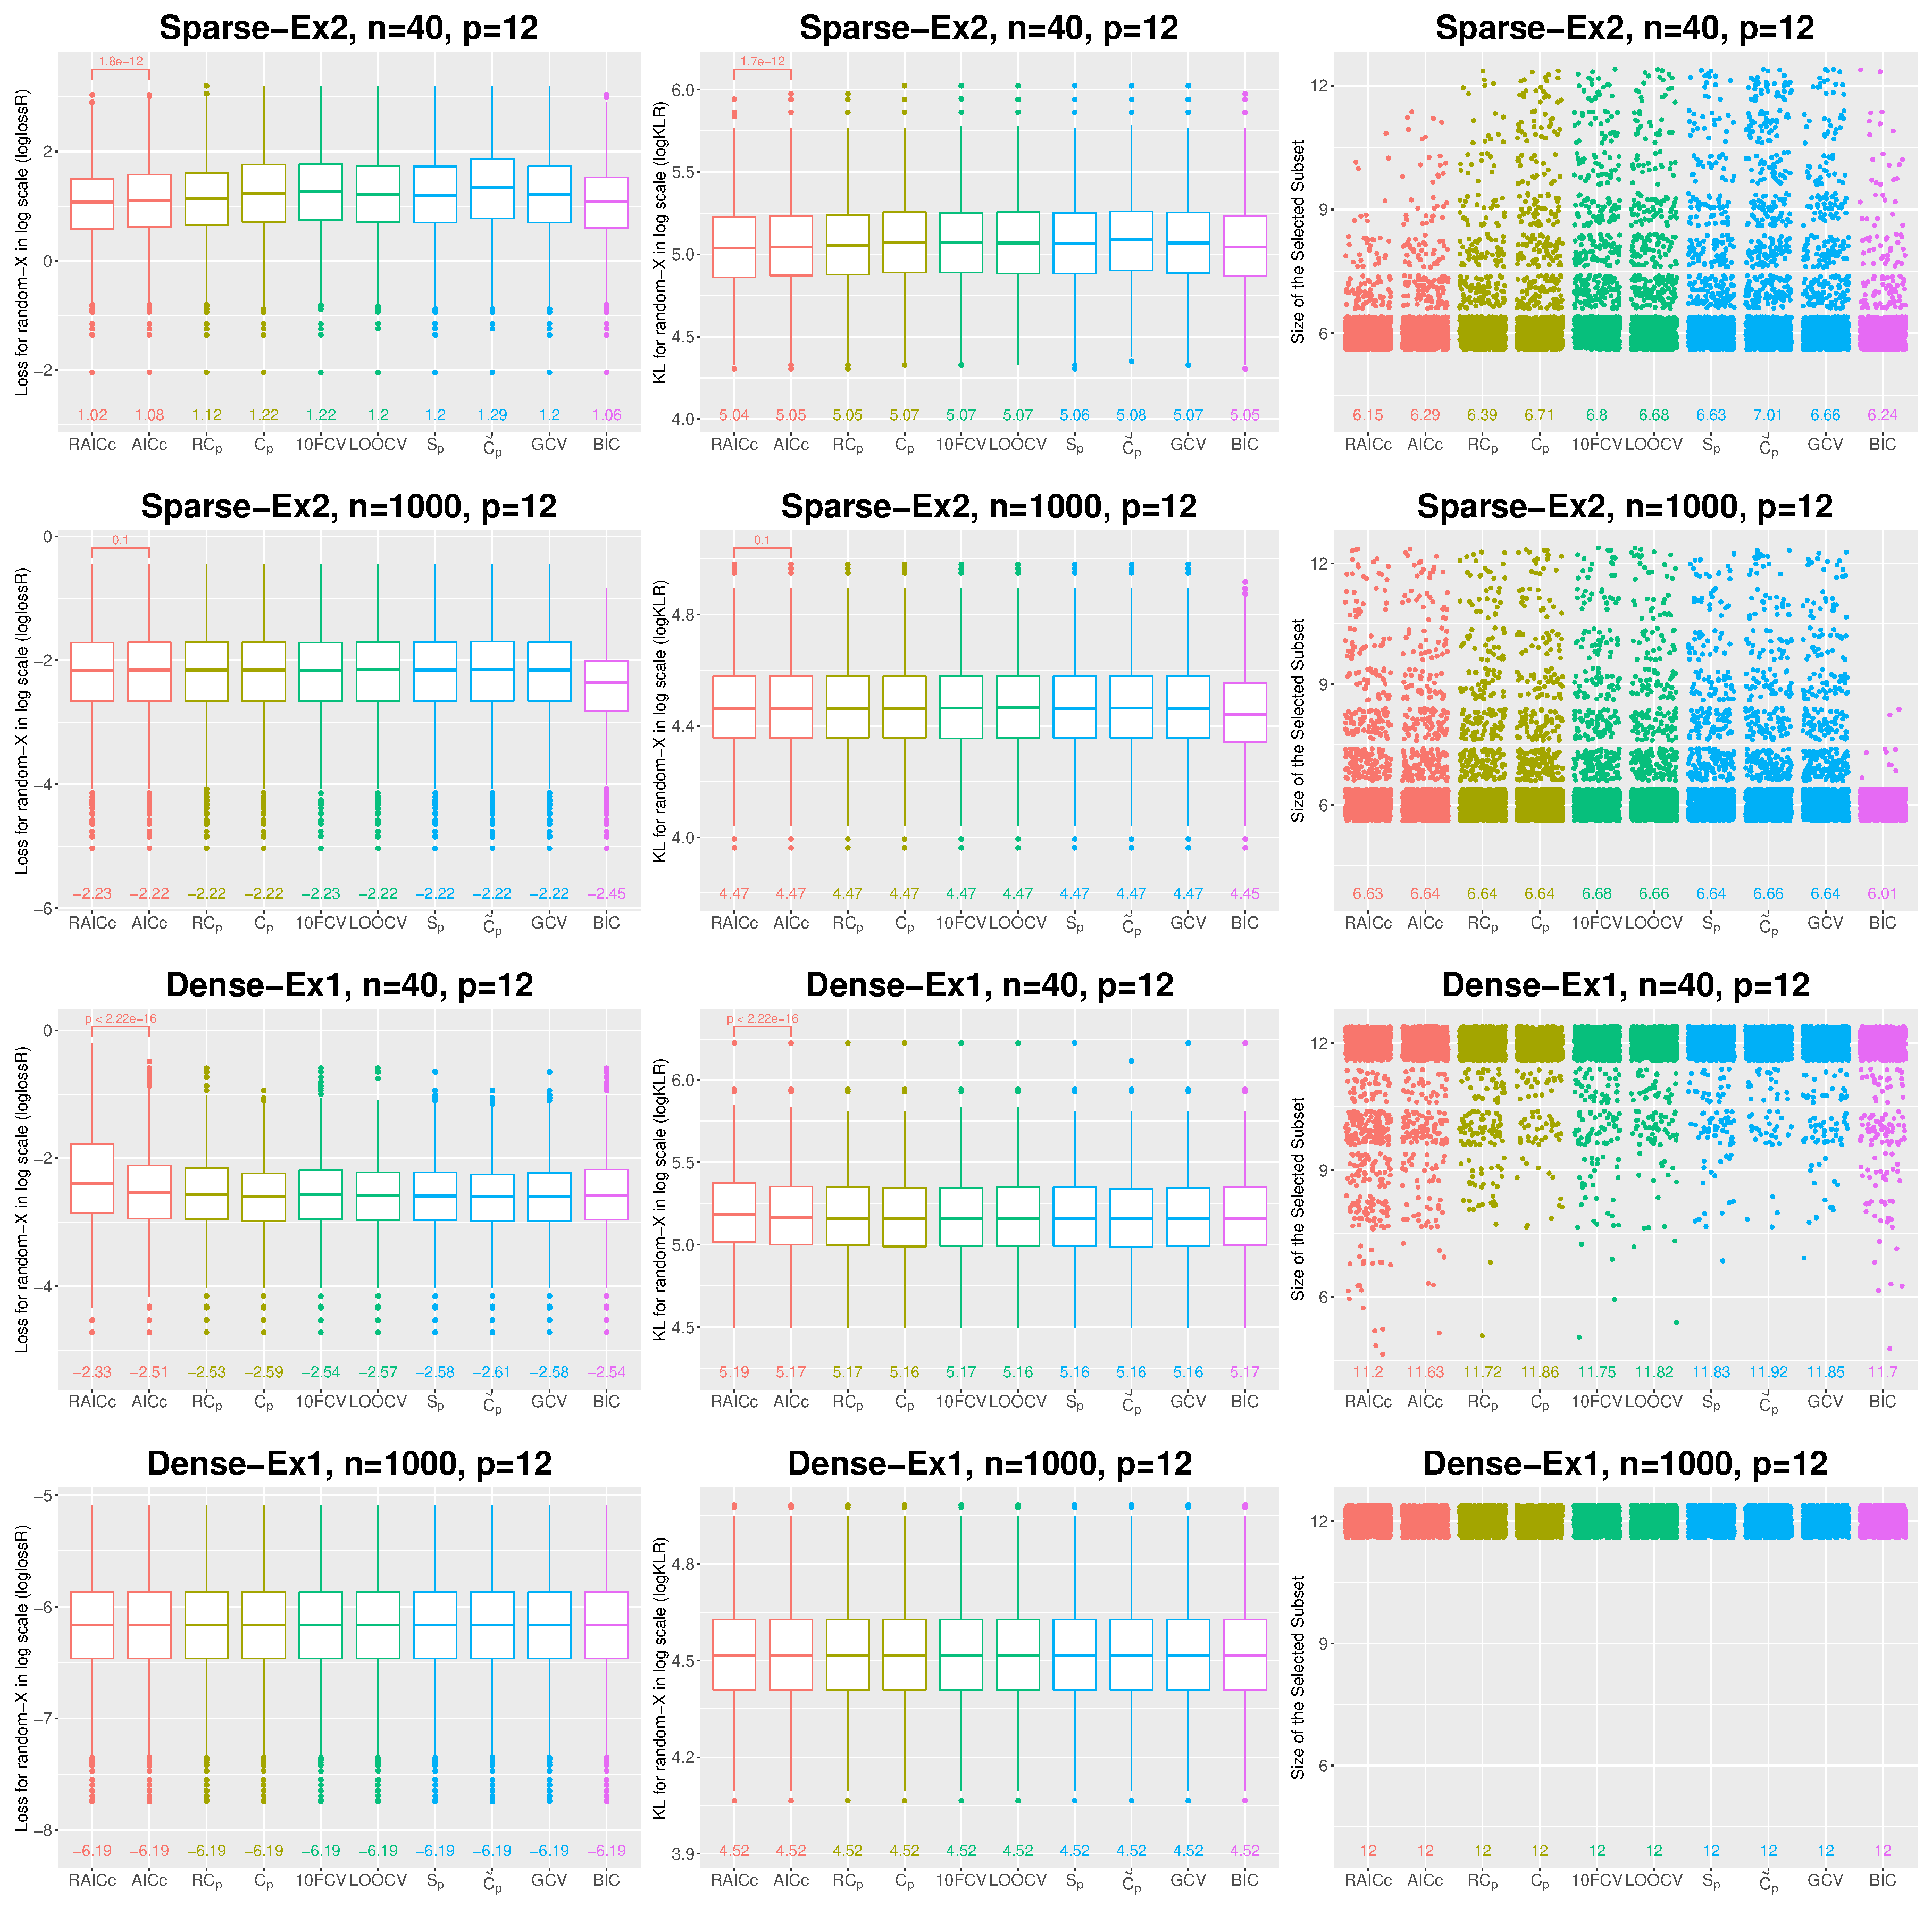
\includegraphics[width=\textwidth]{figures/main/randomx/subset_selection/smallp_hsnr.eps}
  \caption{Random-X, high signal and $\rho=0.5$. The mean values of the evaluation metrics for each criterion are presented at the bottom of each graph. The p-values of the Wilcoxon signed-rank test (paired and two-sided) for comparing RAICc and AICc are also presented.}
  \label{fig:subsetselection_randomx_hsnr_smallp}
\end{figure}

\begin{figure}[!ht]
  \centering
  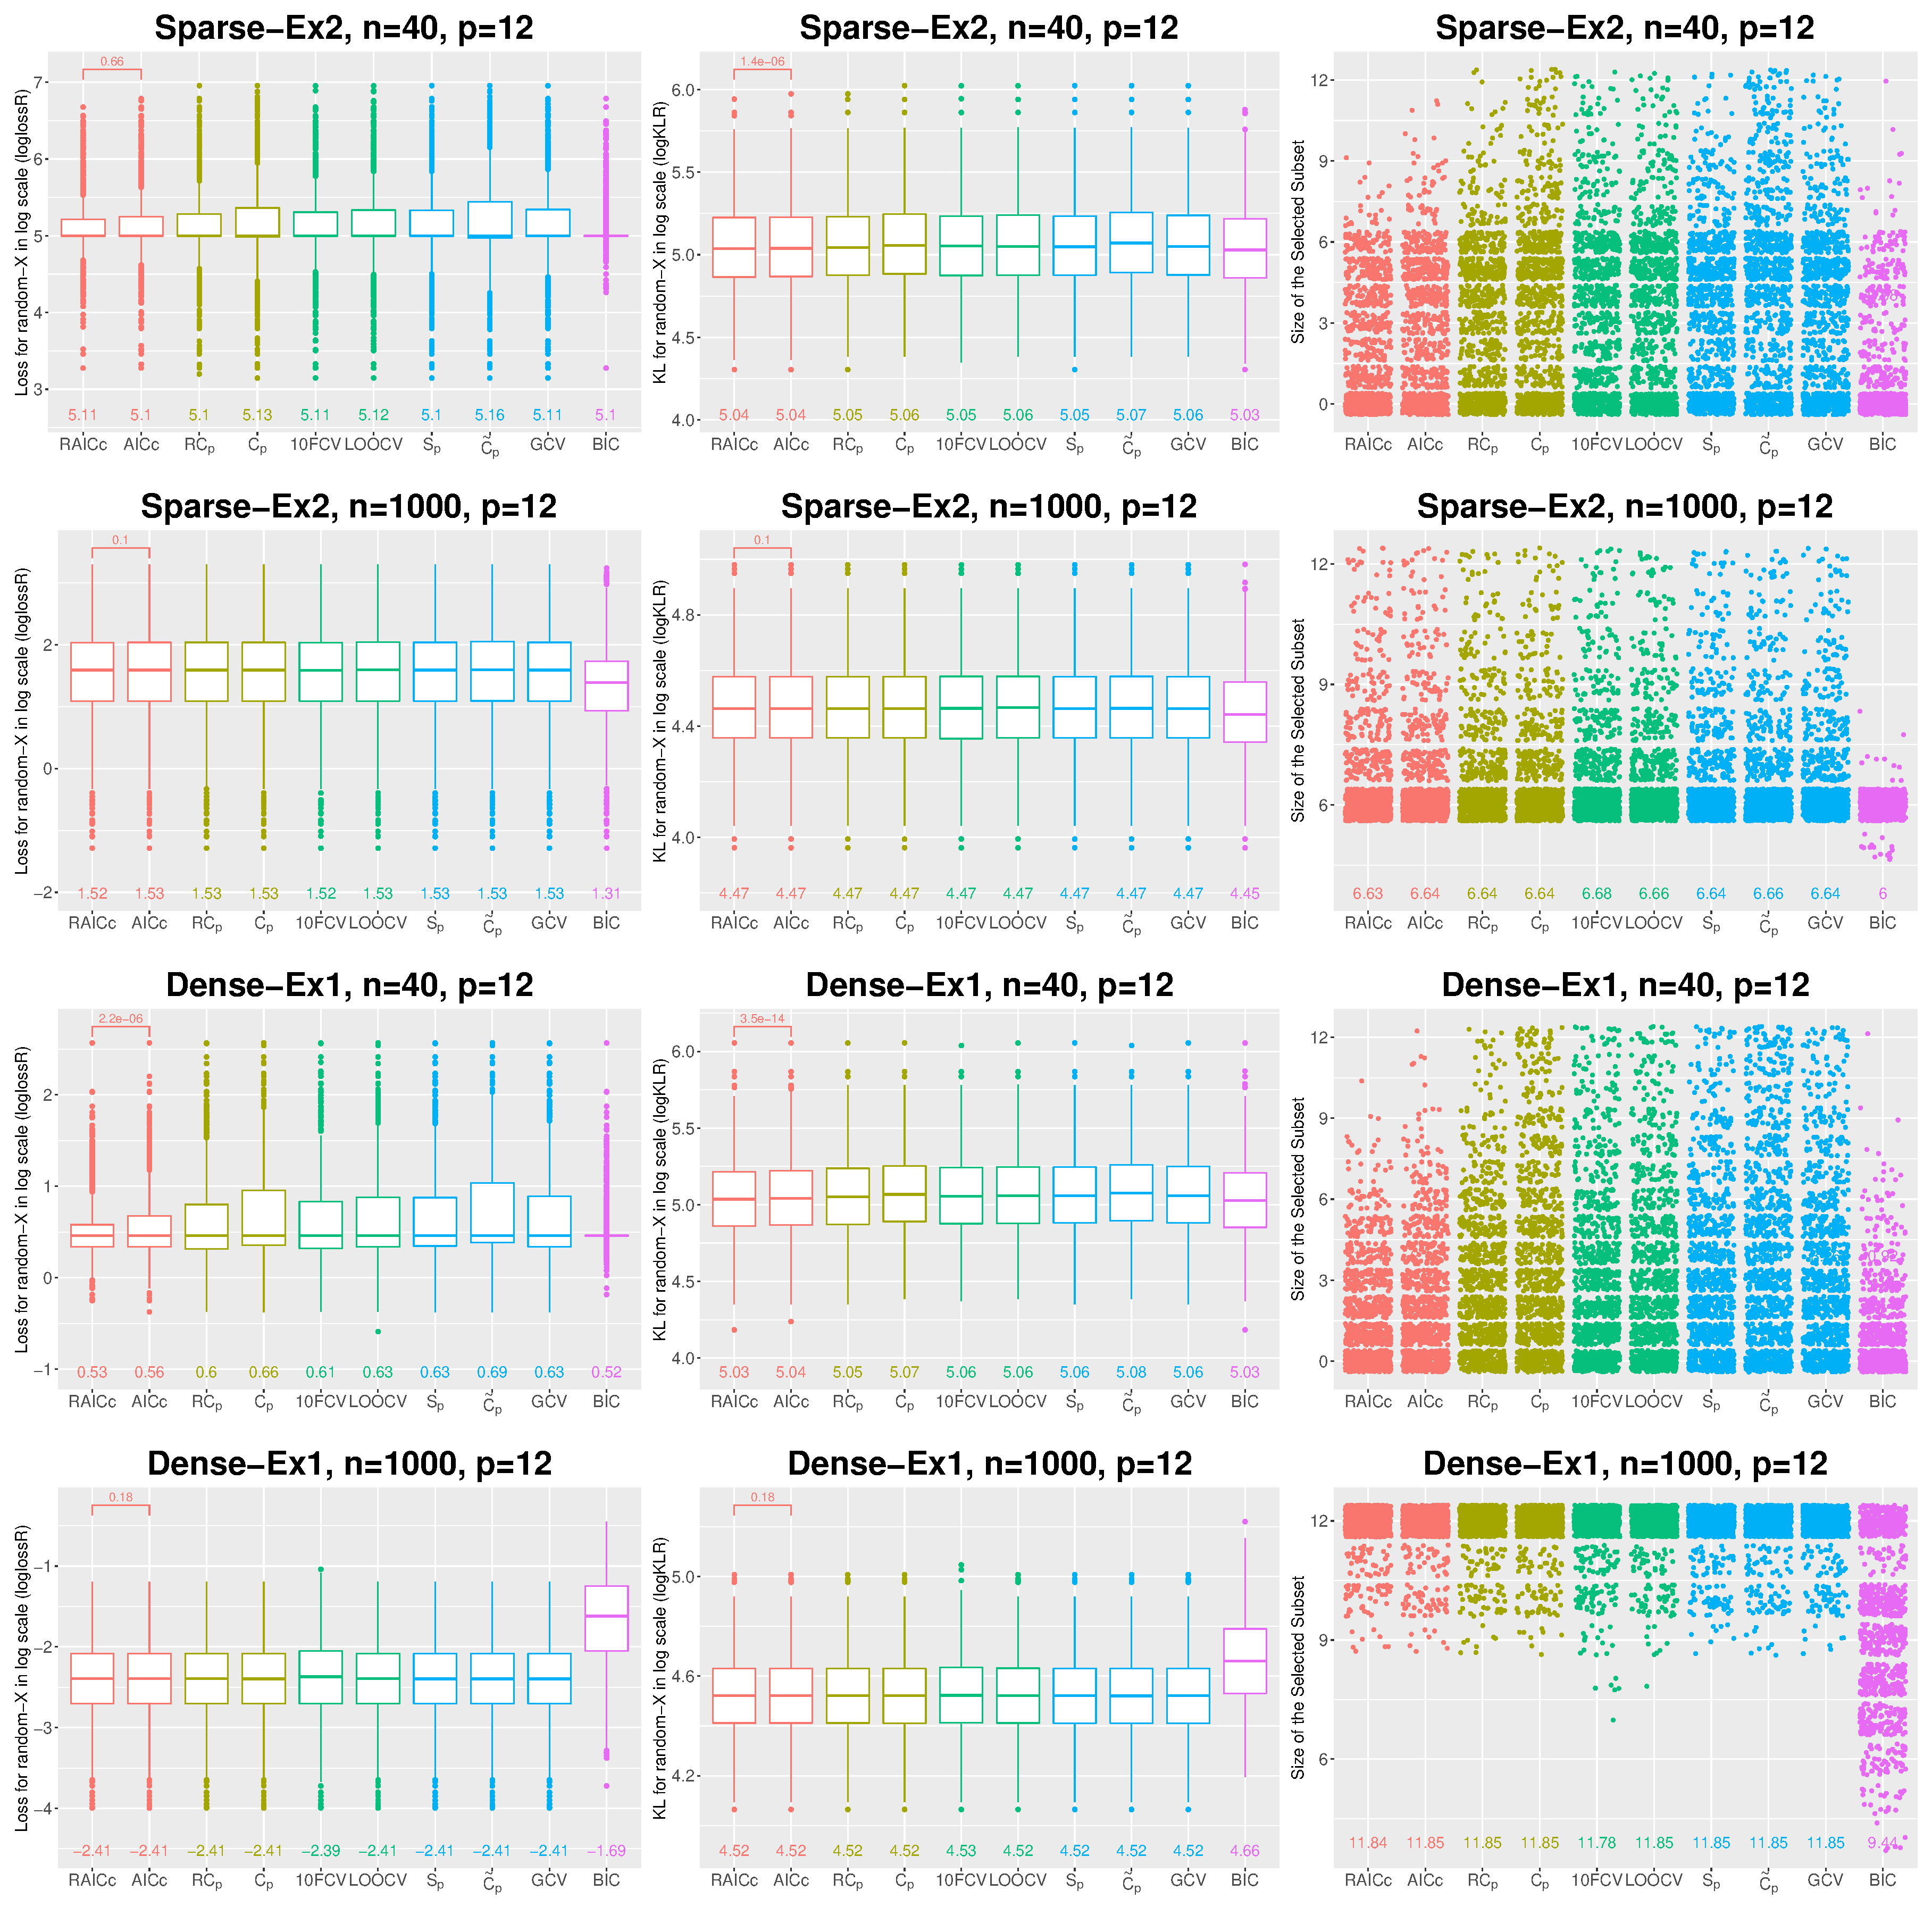
\includegraphics[width=\textwidth]{figures/main/randomx/subset_selection/smallp_lsnr.eps}
  \caption{Random-X, low signal and $\rho=0.5$. Other details are the same as in Figure \ref{fig:randomx_hsnr_smallp}.}
  \label{fig:subsetselection_randomx_lsnr_smallp}
\end{figure}
\fi




\subsection{Fixed-X}
The simulation structure for random-X can also be applied to fixed-X. We only generate the design matrix $X$ once and draw $1000$ replications of the response vector $y$ from the conditional distribution of $y|X$ based on \eqref{eq:truemodel}. The evaluation metrics for fixed-X are as follows. The complete simulation results are given in the Online Supplemental Material. 
\begin{itemize}
  \item Root mean squared error for fixed-X:
  \begin{equation*}
    \text{RMSEF} = \sqrt{ \frac{1}{n}\lVert X\hat\beta-X\beta_0 \rVert_2^2 }.
  \end{equation*} 

  \item KL discrepancy for fixed-X \eqref{eq:KLF} in the log scale (denoted as logKLF).

  \item Size of the subset selected for variable selection problem, and number of restrictions in the selected model for general restriction problem.
\end{itemize}

The patterns for the fixed-X scenario are similar to those for random-X, as can be seen in Figures \ref{fig:subsetselection_fixedx_hsnr_largep}, \ref{fig:subsetselection_fixedx_lsnr_largep}, \ref{fig:generalrestriction_fixedx} and \ref{fig:subsetgeneral_fixedx}. In some ways this is surprising, in that the random-X versions of the criteria still seem to outperform the fixed-X versions, even though that is not the scenario for which they are designed. This seems to be related to the tendency for the fixed-X versions to overfit (or choose too few restrictions) compared to their random-X counterparts, which apparently works against the goal of selecting the candidate with best predictive performance. Otherwise, the KL-based criteria (RAICc and AICc) noticeably outperform the other criteria in general, especially $\mbox{C}_p$ and FPE, particularly for small samples.

\begin{figure}[!ht]
  \centering
  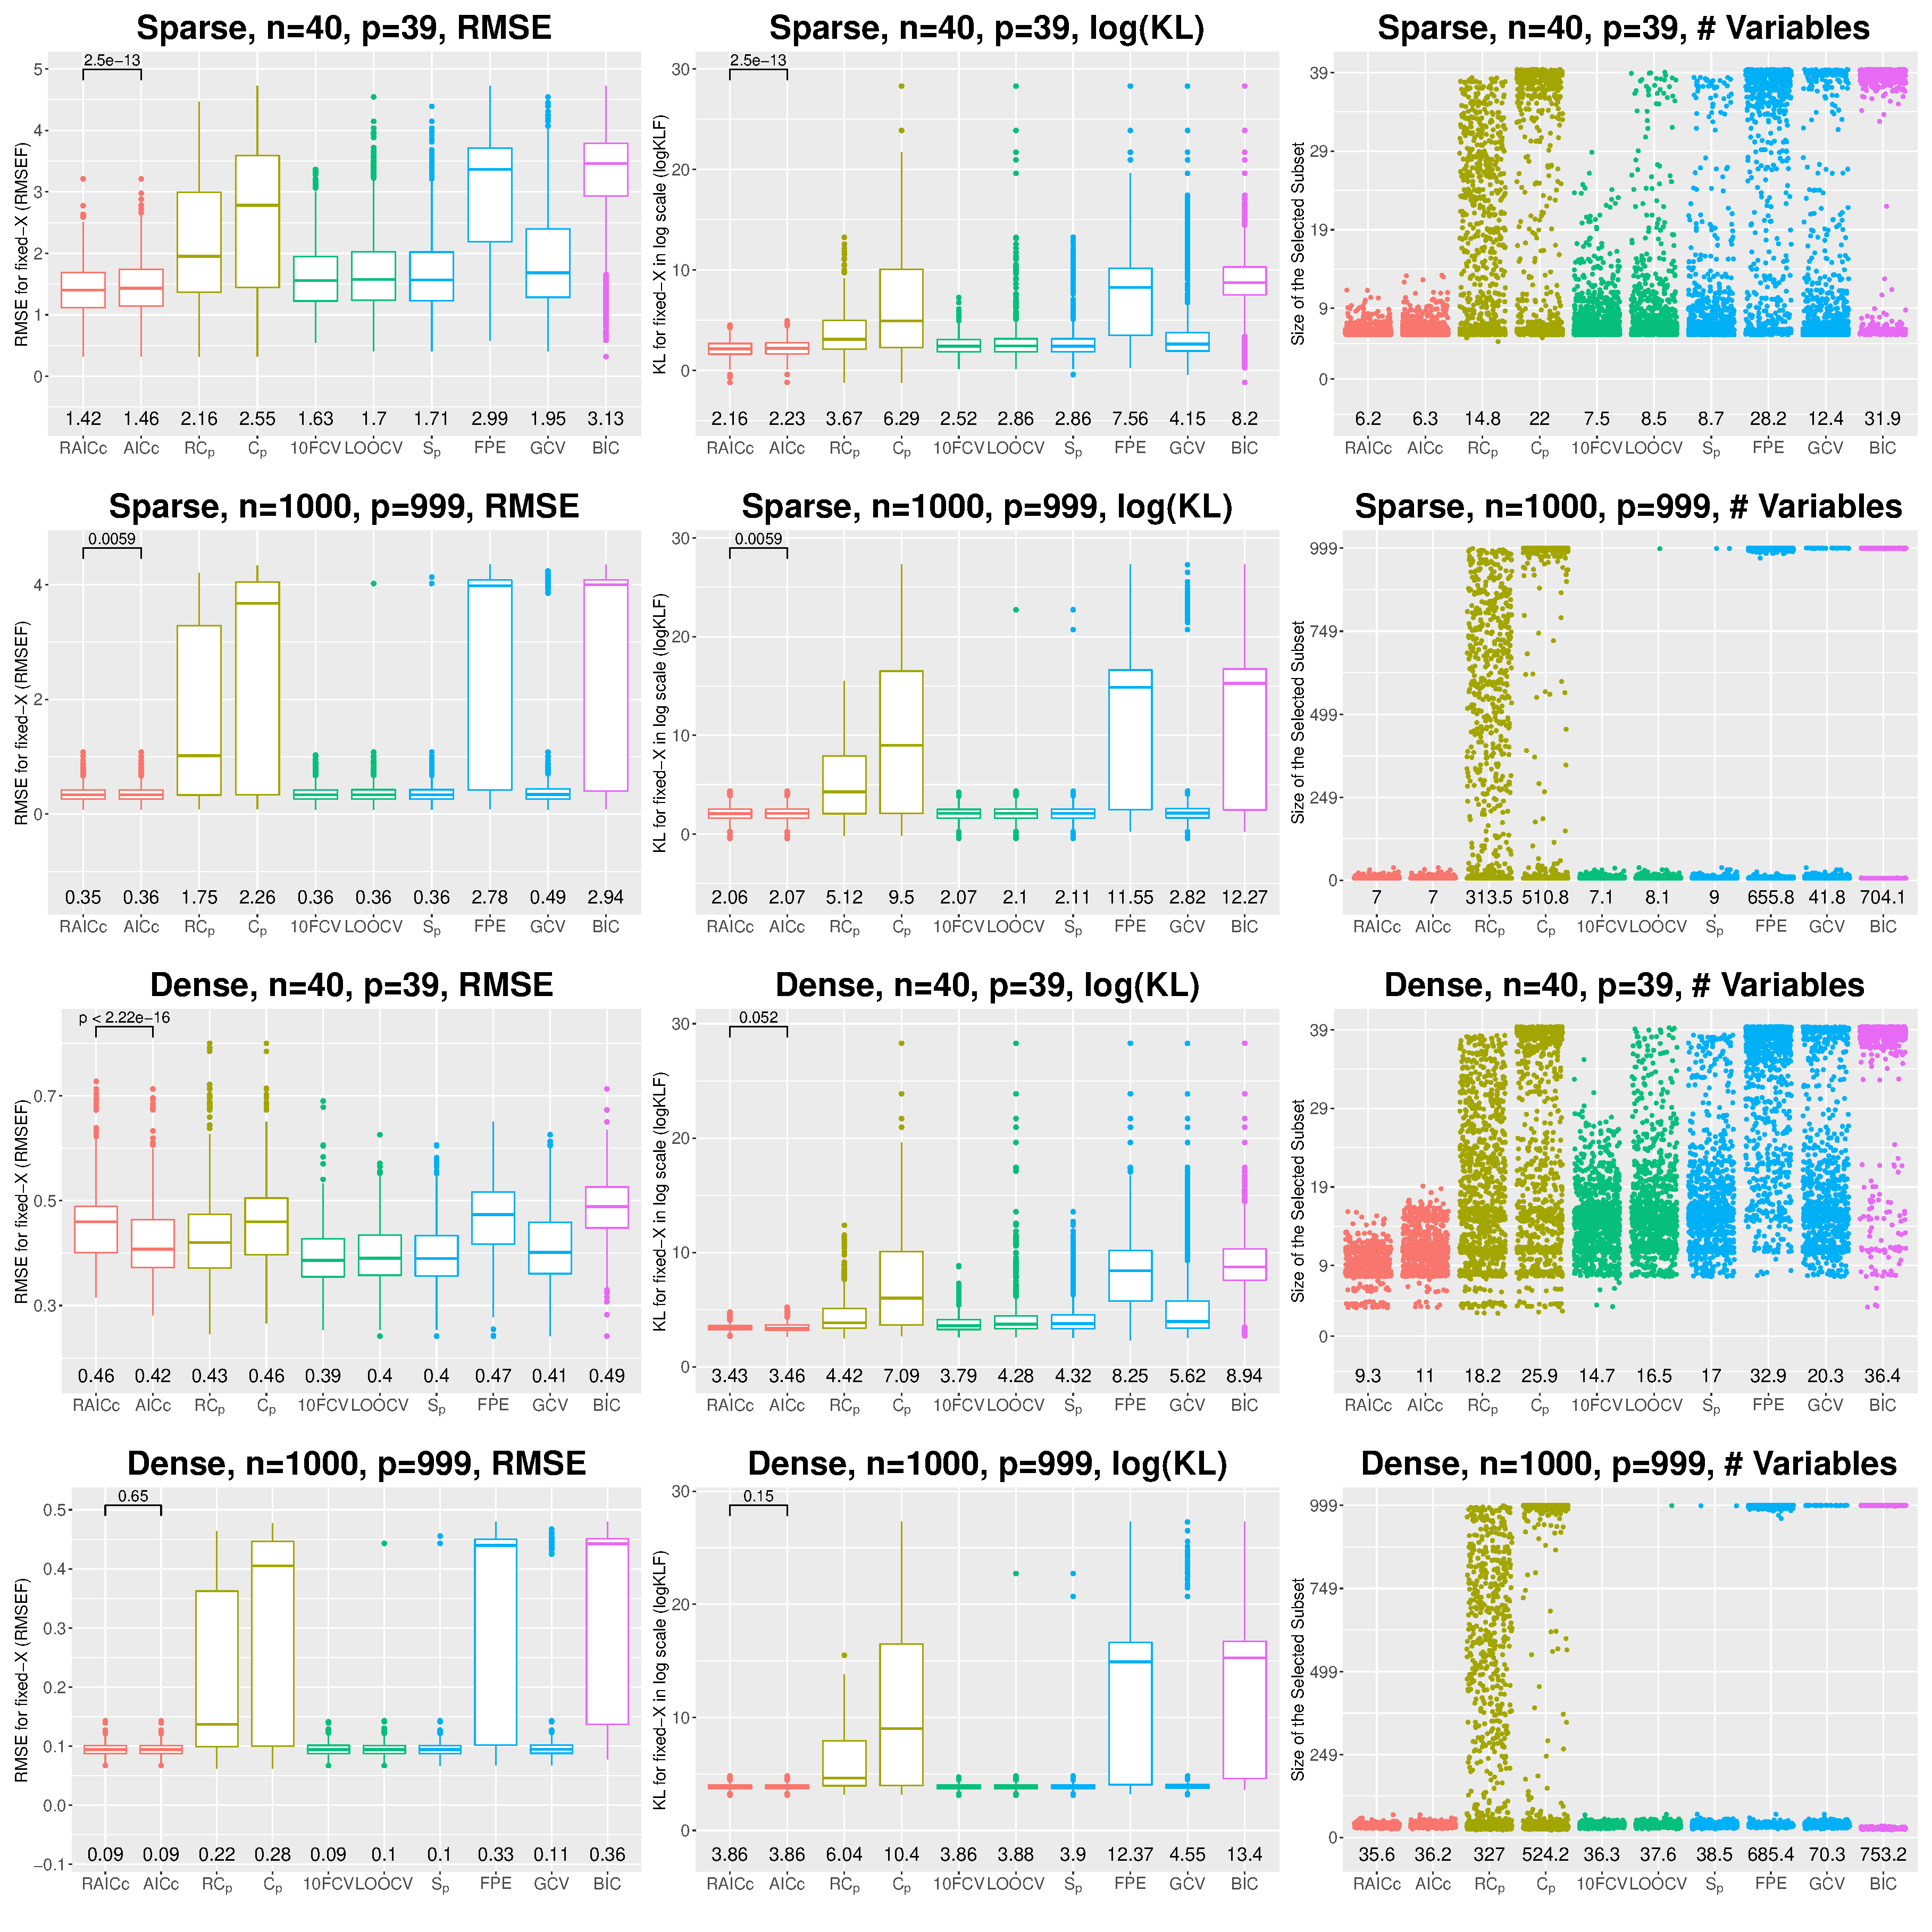
\includegraphics[width=\textwidth]{figures/main/fixedx_VS_hsnr.eps}
  \caption{Results of simulations for variable selection. Fixed-X, high signal. The configurations are the same as in Figure \ref{fig:subsetselection_randomx_hsnr_largep}.}
  \label{fig:subsetselection_fixedx_hsnr_largep}
\end{figure}


\begin{figure}[!ht]
  \centering
  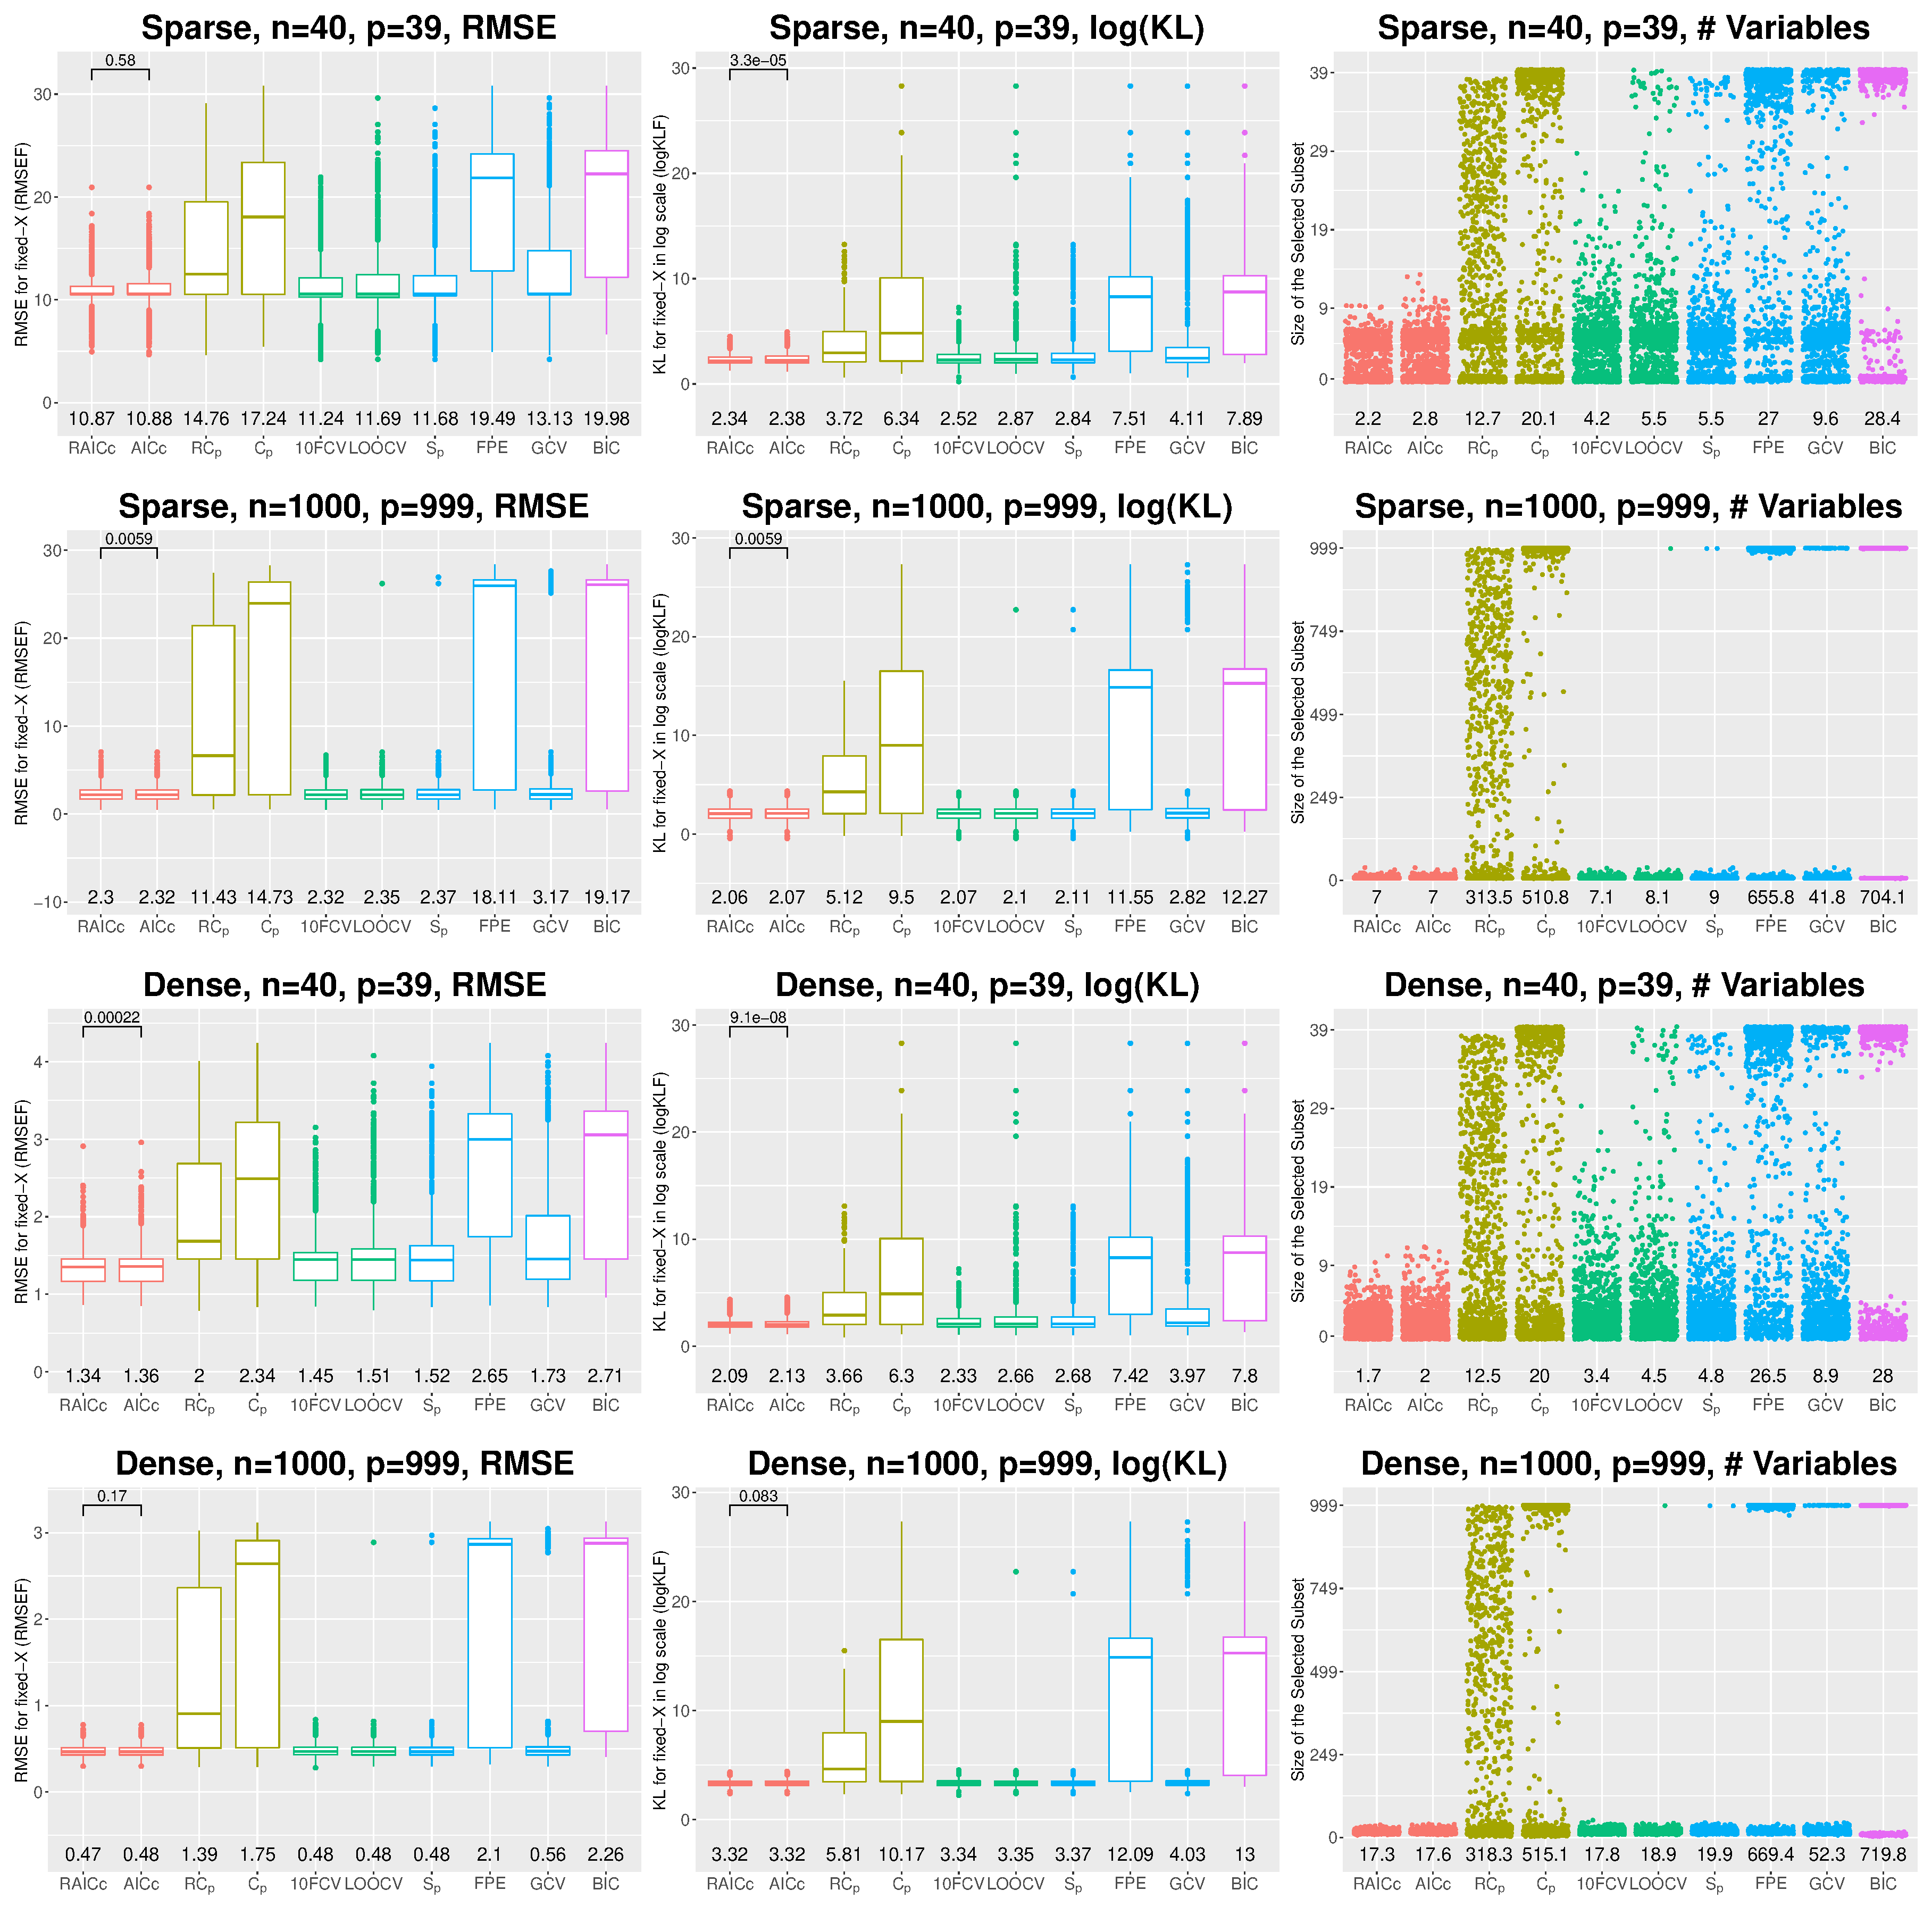
\includegraphics[width=\textwidth]{figures/main/fixedx_VS_lsnr.eps}
  \caption{Results of simulations for variable selection. Fixed-X, low signal. The configurations are the same as in Figure \ref{fig:subsetselection_randomx_lsnr_largep}.}
  \label{fig:subsetselection_fixedx_lsnr_largep}
\end{figure}

\begin{figure}[!ht]
  \centering
  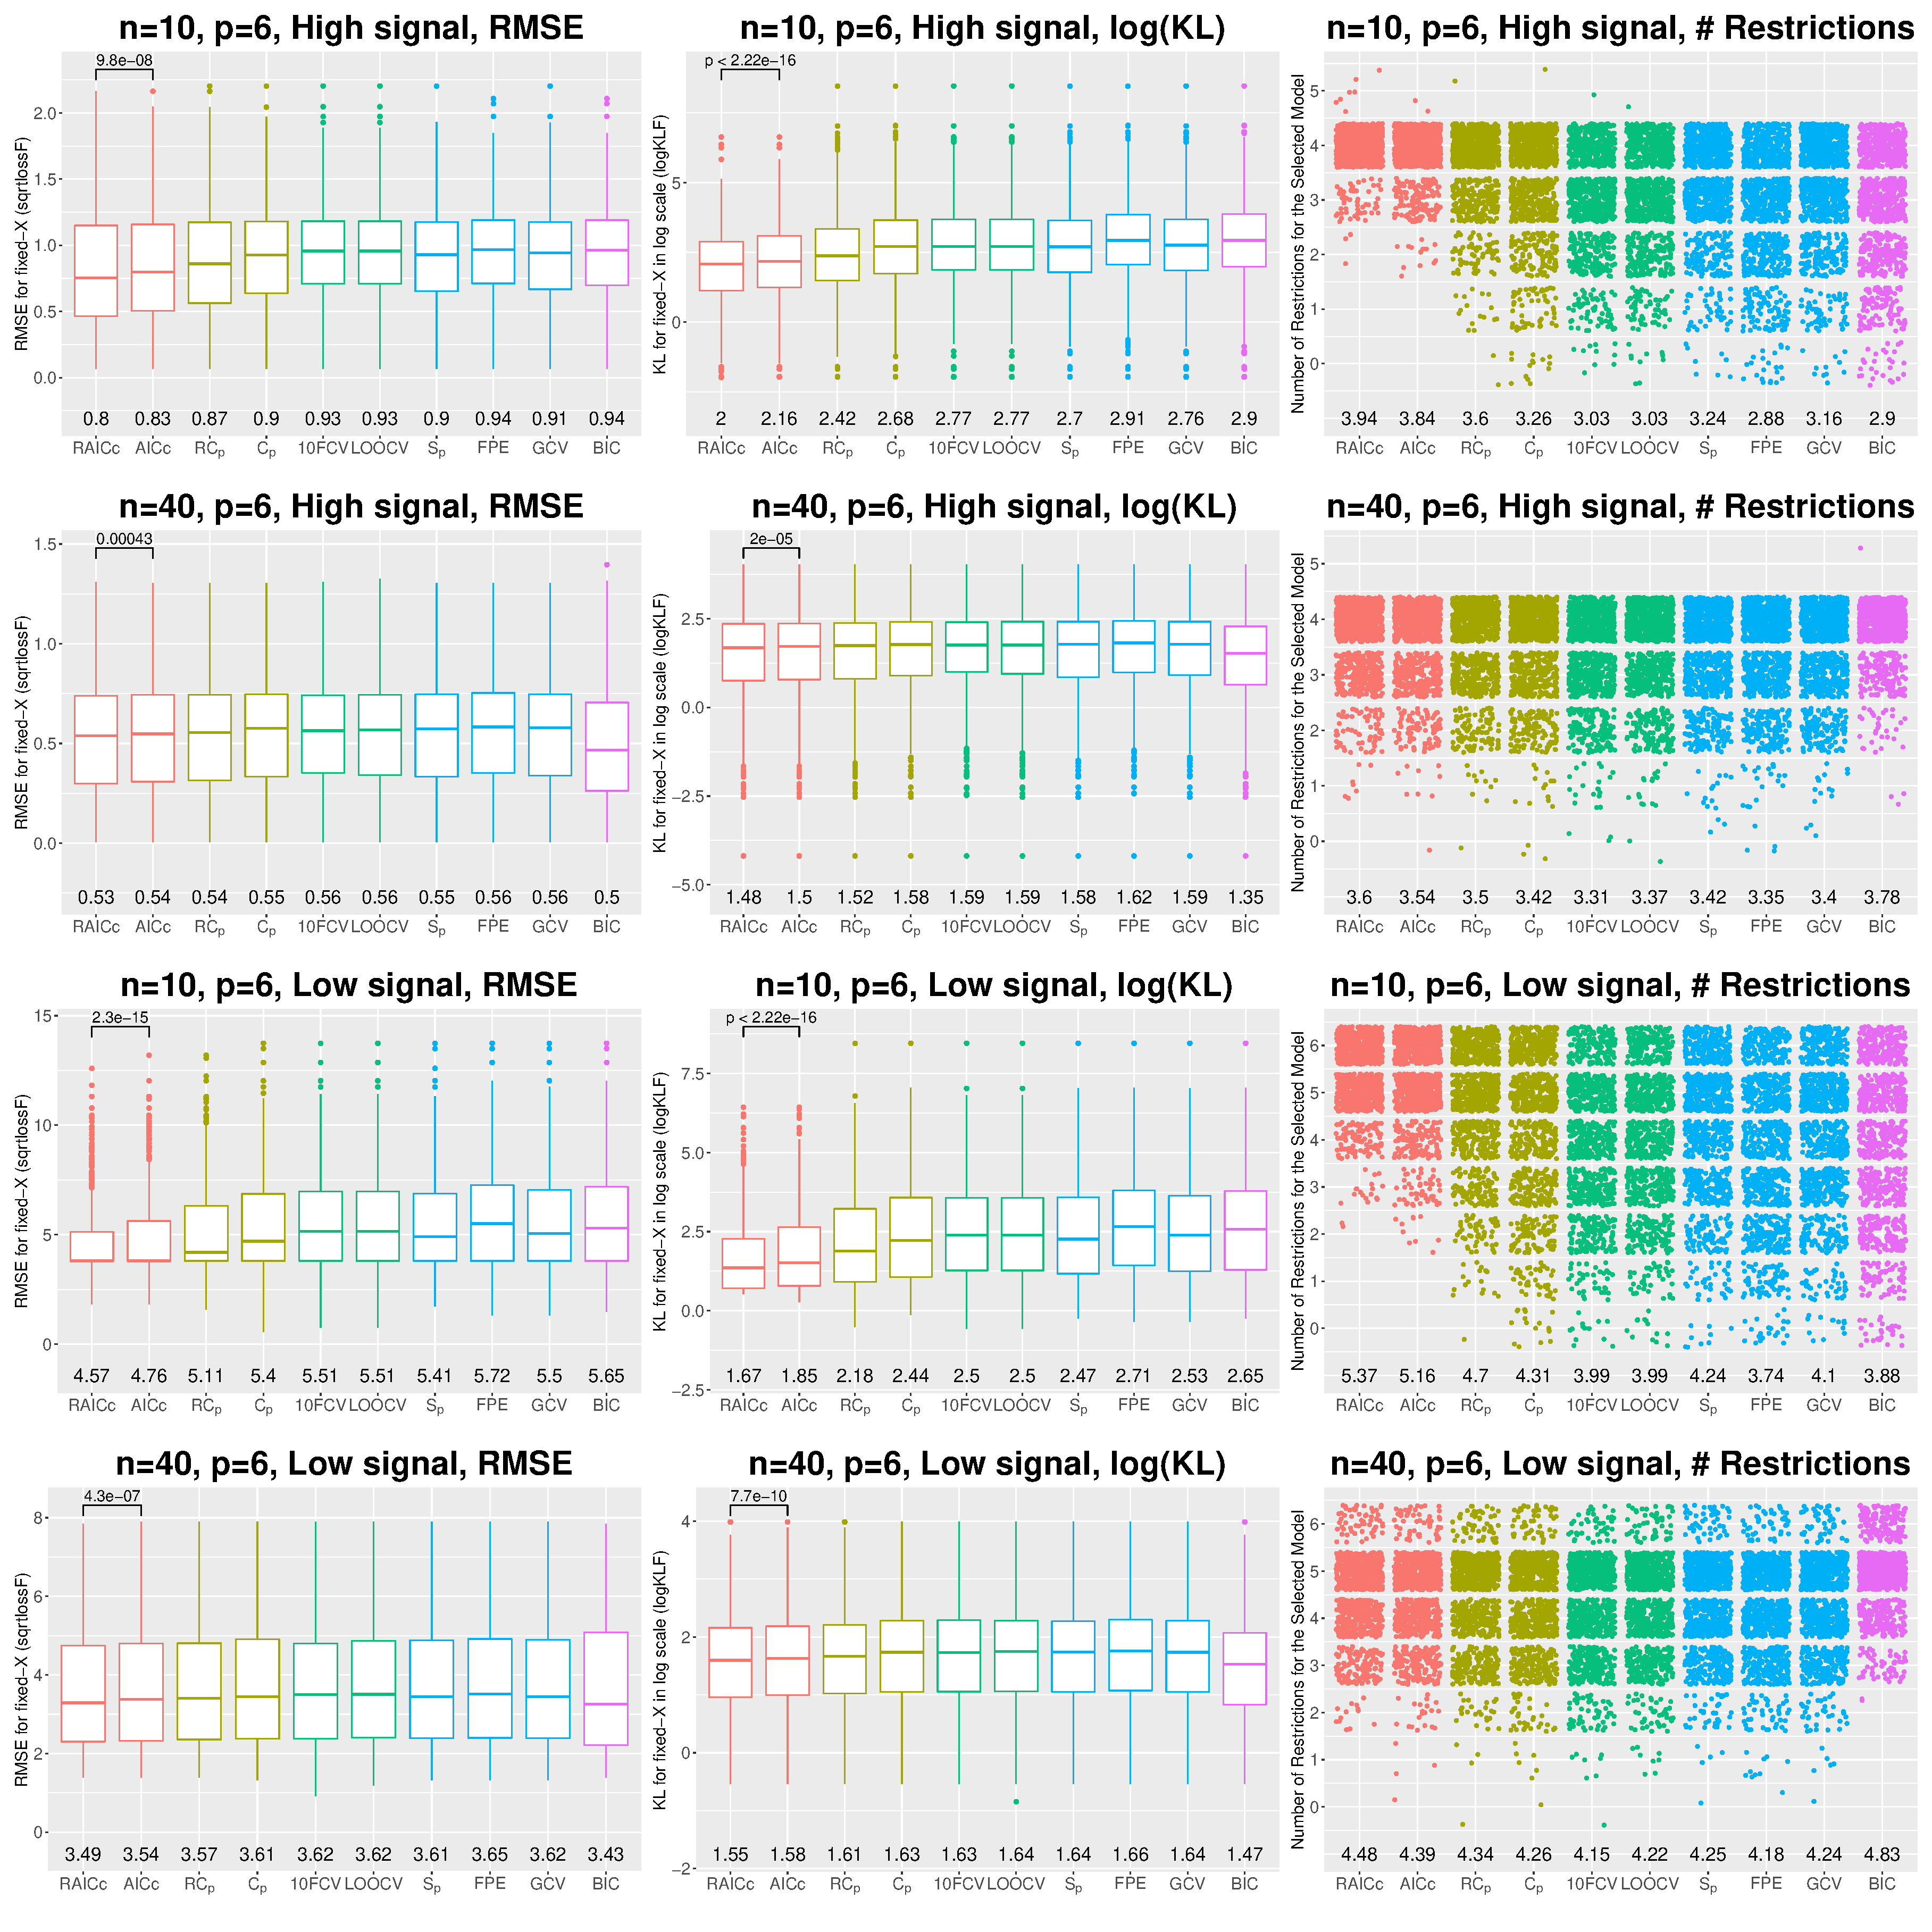
\includegraphics[width=\textwidth]{figures/main/fixedx_GR-Ex1.eps}
  \caption{Results of simulations for general restrictions. Fixed-X, GR-Ex1, $\rho=0.5$. The configurations are the same as in Figure \ref{fig:generalrestriction_randomx}.}
  \label{fig:generalrestriction_fixedx}
\end{figure}

\begin{figure}[!ht]
  \centering
  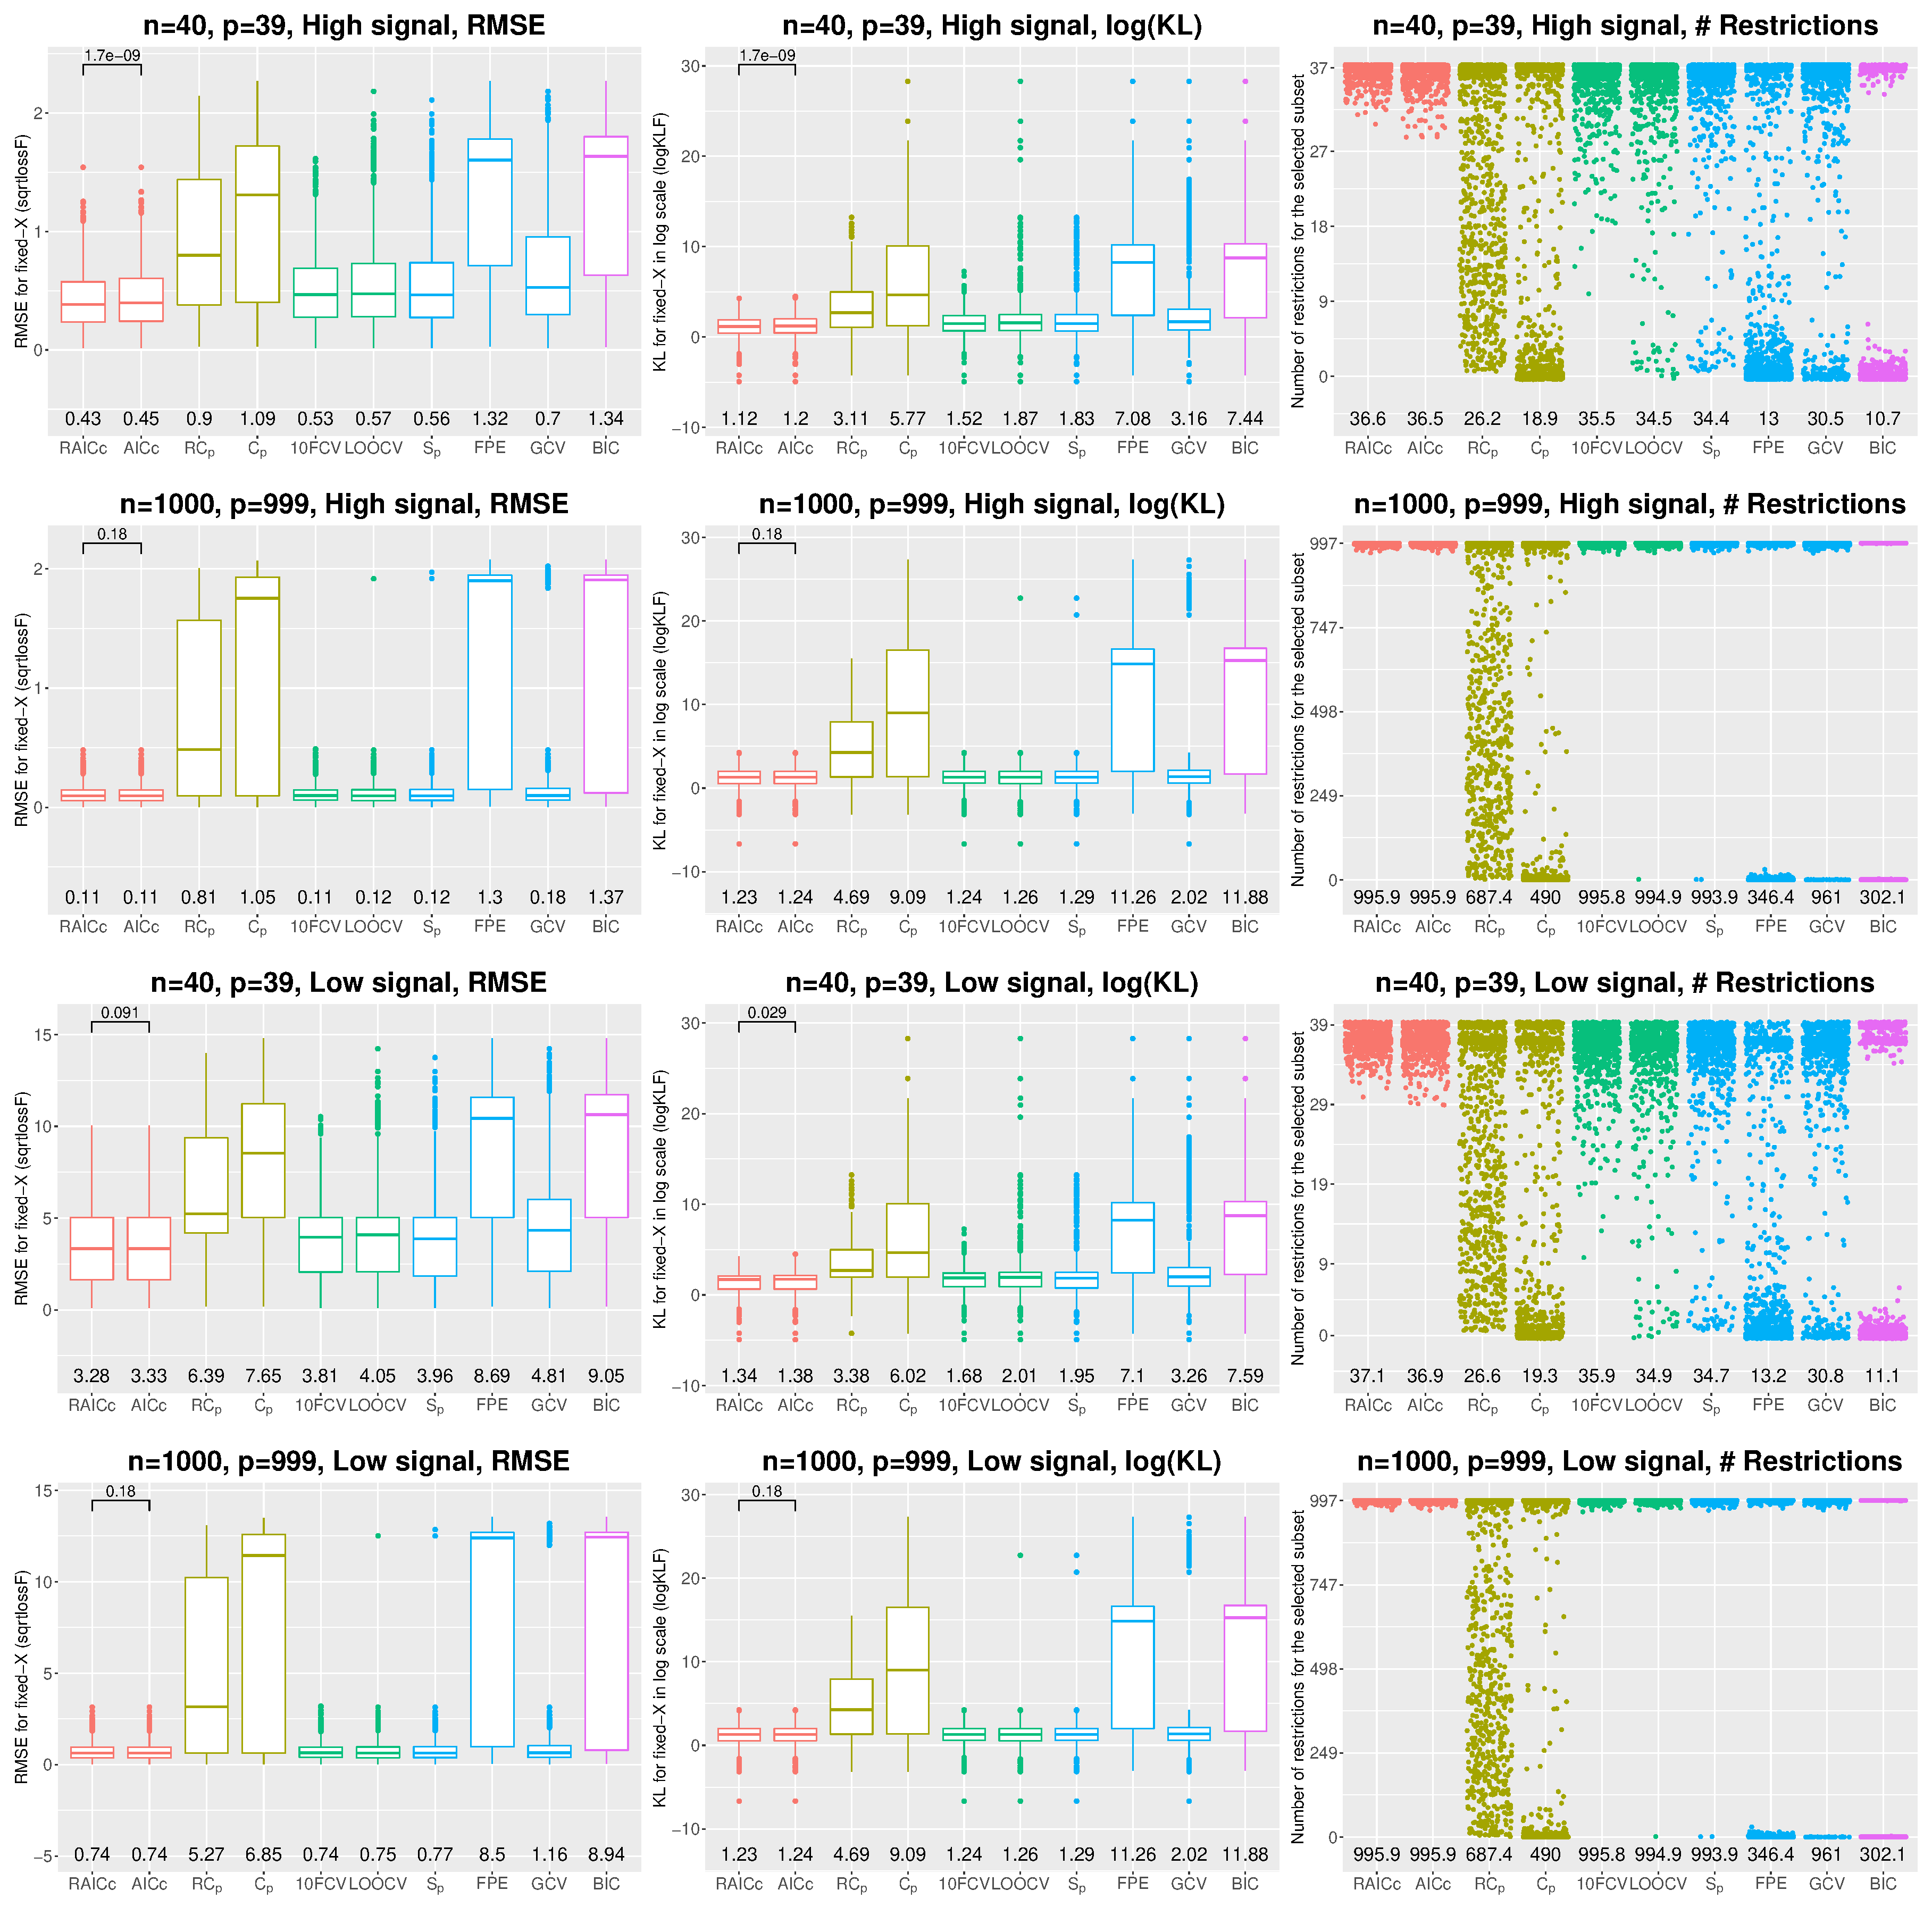
\includegraphics[width=\textwidth]{figures/main/fixedx_GR-Ex4.eps}
  \caption{Results of simulations for general restrictions. Fixed-X, GR-Ex4, $\rho=0.5$. The configurations are the same as in Figure \ref{fig:subsetgeneral_randomx}.}
  \label{fig:subsetgeneral_fixedx}
\end{figure}